\documentclass[a4paper]{article}
\usepackage[a4paper,pdftex]{geometry}
\usepackage[english]{babel}
\usepackage{amsmath,amsfonts}
\usepackage[pdftex]{graphicx}
\usepackage{epstopdf}
\usepackage{fancyhdr}
\usepackage{lastpage}
\usepackage{setspace}
\usepackage{xcolor}
\usepackage{hyperref}
\usepackage{url}
\usepackage[all]{xy}
\usepackage[toc,page]{appendix}
\usepackage[T1]{fontenc}   

% Page margins
%\setlength{\oddsidemargin}{5mm}
%\setlength{\evensidemargin}{5mm}

% Page style
\pagestyle{fancy}

% Page numbering
\lhead{Sensor Fusion on a mini Unmanned Vehicle}
\cfoot{}
\rfoot{\thepage}

% TITLE FORMAT
\newcommand{\HRule}[1]{\rule{\linewidth}{#1}}
% BIBLIOGRAPHY

\makeatletter
\def\printtitle{
    {\centering \@title\par}}
\makeatother                  

\makeatletter
\def\printauthor{
    {\centering \large \@author}}
\makeatother

% TITLE
\title{
\HRule{0.5pt} \\
\LARGE \textbf{\textsc{Sensor Fusion on a mini Unmanned Vehicle}}\\[0.5cm]
\normalsize \textsc{Integrating vision-based algorithms on an Parrot AR.Drone to autonomously follow linear shaped structures in a landscape.}
\HRule{2pt}\\ [0.5cm]
Camiel R. Verschoor\\
10017321\\
\vspace{1cm}
Bachelor thesis\\
Credits: 18 EC\\
\vspace{0.5cm}
Bachelor Opleiding Kunstmatige Intelligentie\\
\vspace{0.25cm}
University of Amsterdam\\
Faculty of Science\\
Science Park 904\\
1098 XH Amsterdam\\
}

% AUTHOR
\author{\normalsize
\emph{Supervisors}\\
Dr. A. Visser\\
\vspace{0.25cm}
Informatics Institute\\
Faculty of Science\\
University of Amsterdam\\
Science Park 904\\
1098 XH  Amsterdam\\
\vspace{0.5cm}
Drs. G. Poppinga\\
\vspace{0.25cm}
Defense Systems\\
Aerospace Systems\\
National Aerospace Lab\\
Anthony Fokkerweg 2\\
1059 CM Amsterdam\\
\vspace{1cm}
July 24th, 2012\\
}

% BEGIN DOCUMENT
\begin{document}

% TITLE PAGES
\thispagestyle{empty}
\begin{center}
\Large\textsc{Sensor Fusion on a mini Unmanned Vehicle}\\
\normalsize\textsc{Integrating vision-based algorithms on an Parrot AR.Drone to autonomously follow linear shaped structures in a landscape.}

\vspace{2cm}

\begin{figure*}[!ht]
\centering
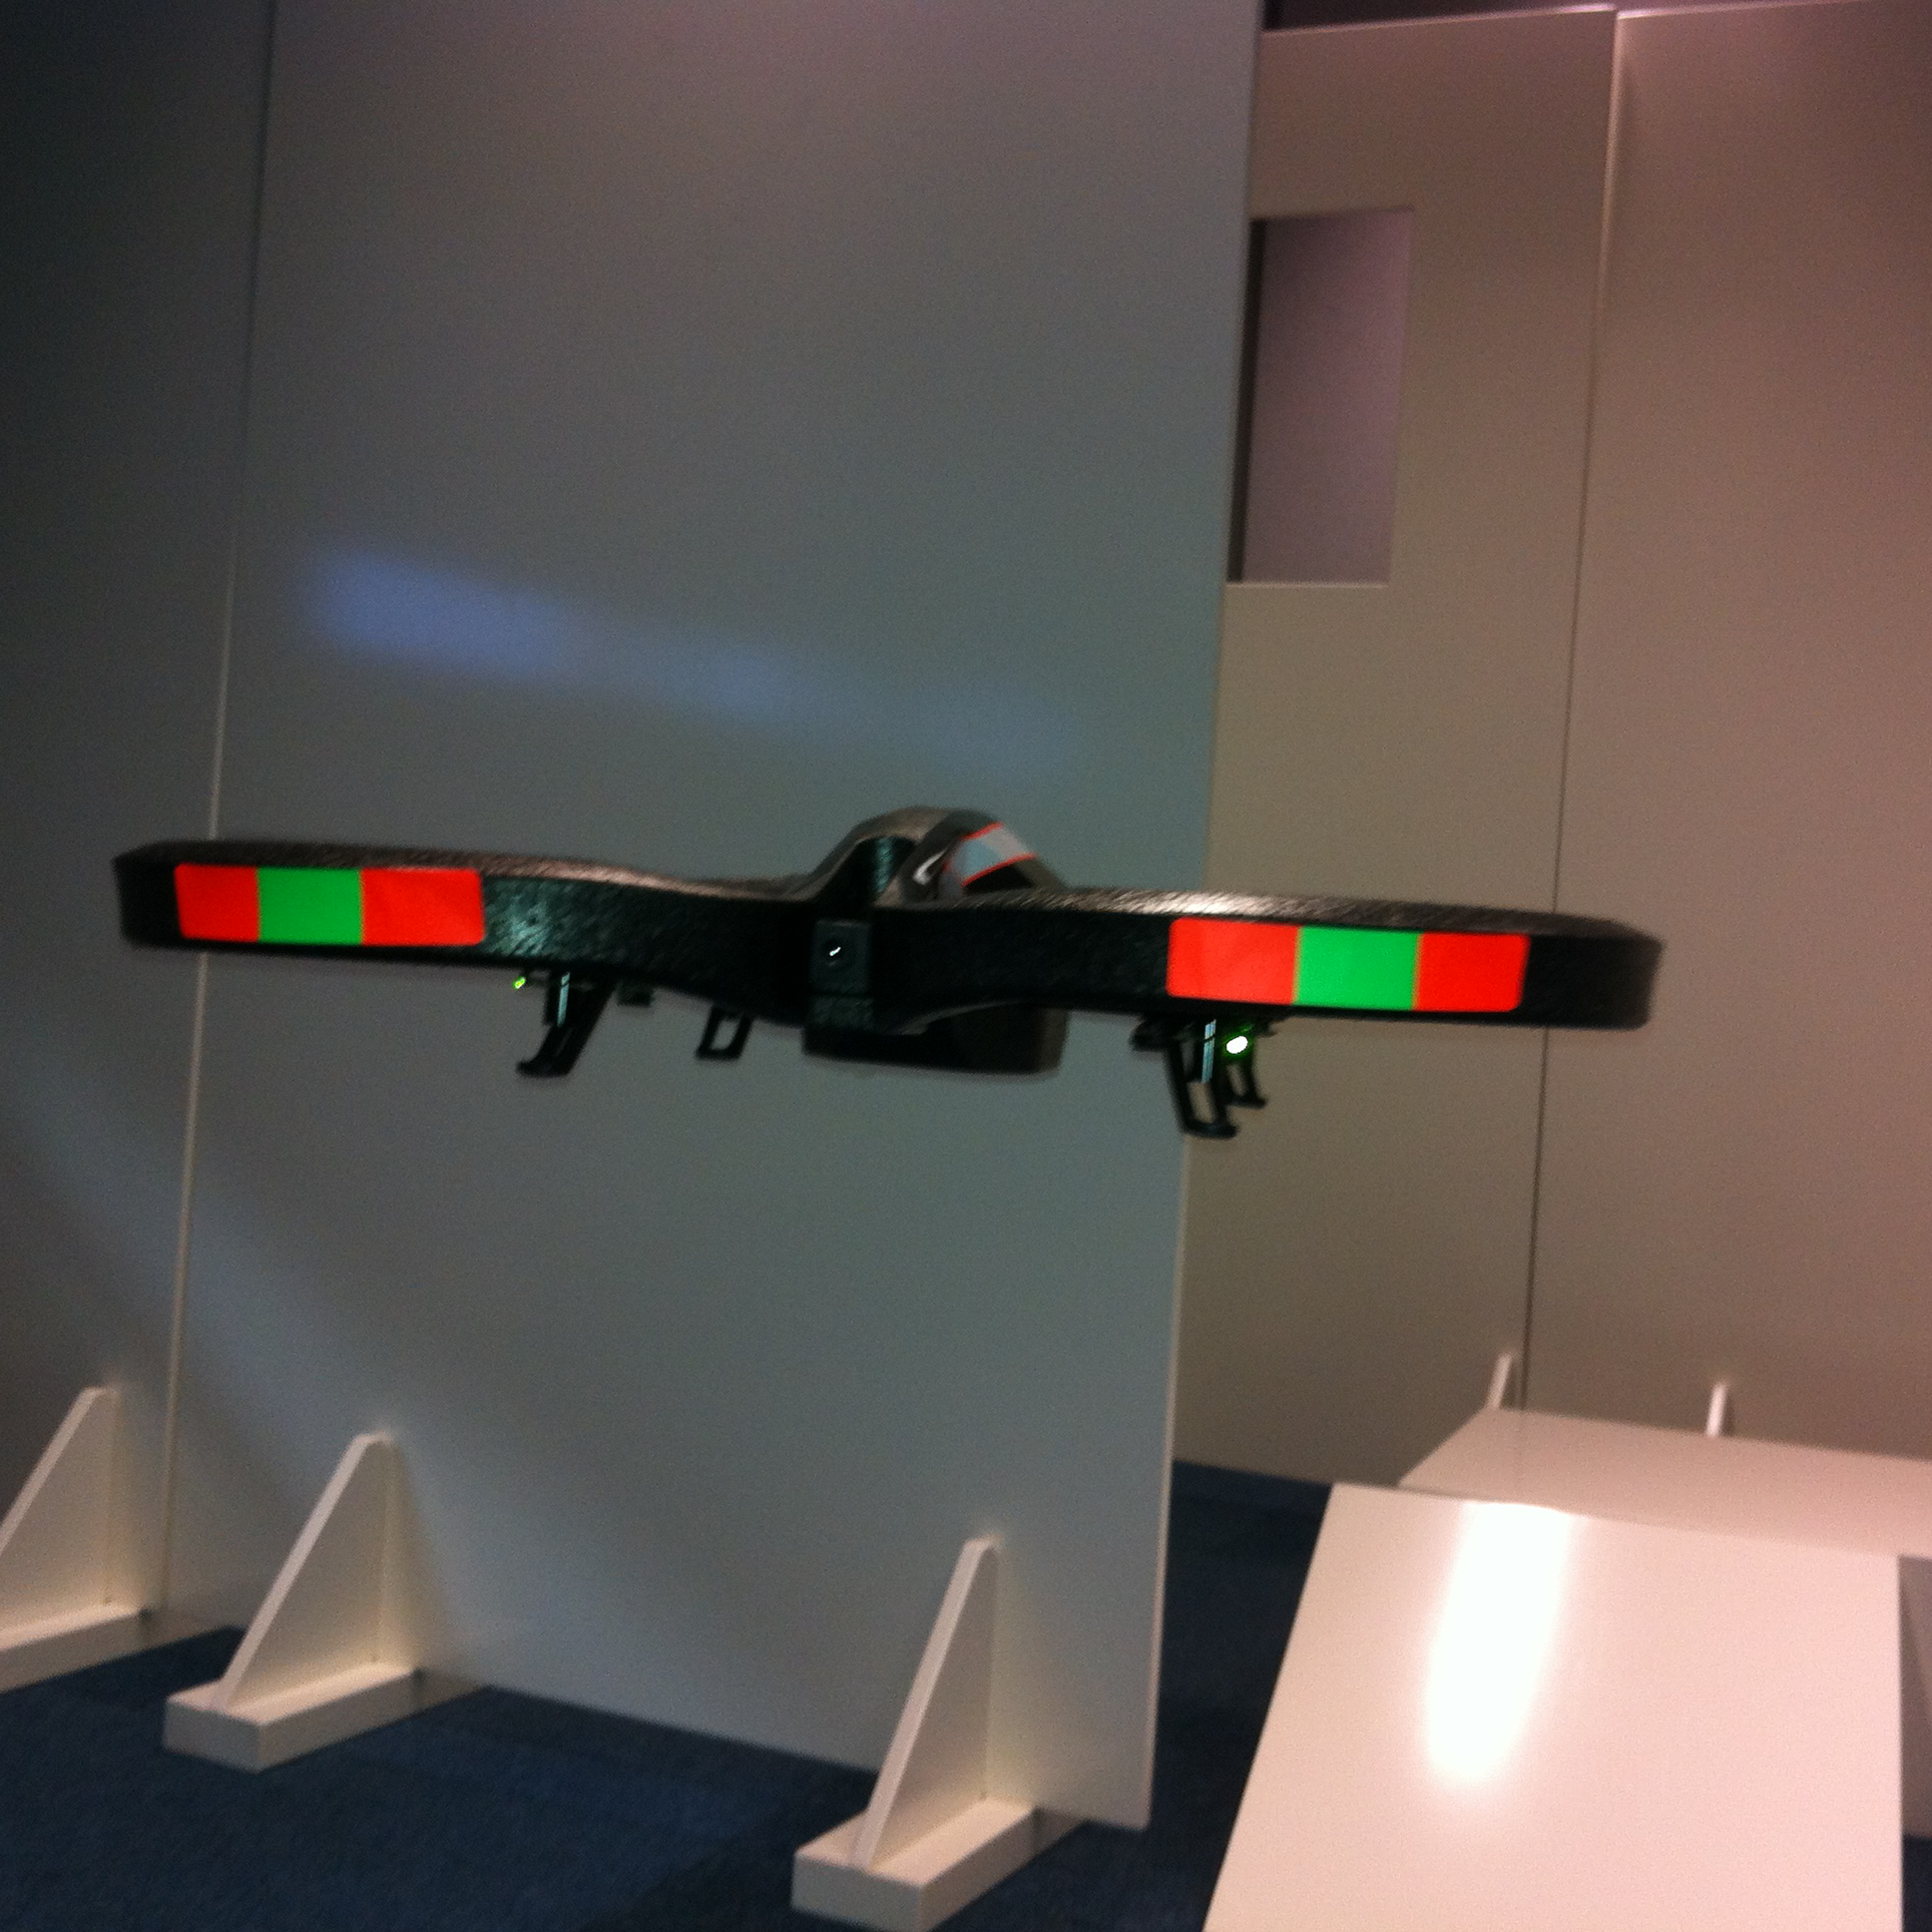
\includegraphics[width=\textwidth]{images/front.png}
\end{figure*}

\subsubsection*{A Bachelor Thesis by Camiel R. Verschoor}
\end{center}
\newpage

% EMPTY PAGE
\thispagestyle{empty}
\mbox{}
\newpage

% THESIS INFORMATION
\thispagestyle{empty}
\printtitle
\vfill          
\printauthor
\newpage

% ABSTRACT
\thispagestyle{empty}
\begin{abstract}
One of the main requirements in enabling autonomous flight of Micro Aerial Vehicles (MAVs) in GPS denied and deprived environments is the ability for navigation. One possible solution to solve this navigation problem is to use a vision-based line-following algorithm since there are various linear structures in the operating environment. Edge and motion detection have proven to be strong algorithms for the detection of objects. However, these detection algorithms have their weaknesses. In order to overcome these weaknesses this thesis proposes a two stage approach, which is a common approach for object recognition. In the first stage edge and motion detection are combined to strengthen each other. In the second stage a Probabilistic Hough Transform (PHT) is performed to extract the line from the pre-processed image PHT determines a directional vector for navigation purposes and can be used to make the platform move accordingly. This thesis is a survey for the experimental circumstances to fairly test both algorithms for a line-following task.
\end{abstract}
\vfill
\section*{Acknowledgements}
I would like to thank my supervisors Arnoud Visser and Gerald Poppinga for their support and guidance. Furthermore, I am grateful to Nick Dijkshoorn for the distribution of his development framework, AR.Drone SLAM, and his support installing it. I also like to thank Robrecht Jurriaans for borrowing his AR.Drone. Likewise, I would like to thank Rob van Holstein for the construction of the 3-Dimensional printed frame of the mirror construction. I like to thank Christian Muller for helping collecting the dataset and learning me to fly a quadcopter manually. Furthermore, I am grateful to the National Aerospace Lab for the internship and the visit to the International Micro Aerial Vehicle Conference and Competitions. Lastly, I am thankful to my girlfriend and my family for their support and encouragement.
\newpage

% TABLE OF CONTENTS
\thispagestyle{empty}
\tableofcontents
\thispagestyle{empty}
\newpage
\setcounter{page}{1}
% SPACING
%\onehalfspace

% INTRODUCTION
\section{Introduction}
In robotics one of the main goals is to develop mobile robots that can operate autonomously in the real world environment. These autonomous robots have various purposes and are used for a wide range of applications such as inspection, exploration and rescue. In rescue, robots are expected to operate in dangerous environments without putting human lives at risk. Even though reasonable developments have been made in the robotics field, robots cannot operate autonomously in the real world yet.

One of the main requirements of an autonomous robot is the ability of navigation in the operational environment. The traditional approach to navigate through the outdoor environment is via pre-planned paths based on a Global Positioning System (GPS). The main shortcoming of GPS is that it cannot be used in every environment as it needs to receive data signals from at least four different satellites \cite{Bajaj2002}. Inside buildings and in several outdoor areas GPS is not convenient for navigation. In urban areas GPS is found to be especially unreliable. In order to navigate through these environments other sensors and navigation techniques need to be applied. Since there are several linear structures in the environment such as rivers, roads and power lines, line-following is one possible approach to navigate through an environment. Line-following is a classic technique in robotics as it has been successfully used for ground robots numerous times \cite{Sampei1995, Dupuis2006}. For other robots and sensor configurations, open problems still remain. One of these is navigation for micro aerial vehicles (MAVs), which have a limited sensor composition due to their limited payload. For MAVs line-following is a greater challenge due to the extra dimension it can move in, comparing to the average ground robot. Where the sensors of a ground robot can rely on the stability of the ground, the sensors of a MAV have to count on the stability of the platform during a flight. Therefore, MAV are more likely to measure noisy data, which interpreting algorithms should be able to handle.

\begin{figure}[!ht]
	\centering
	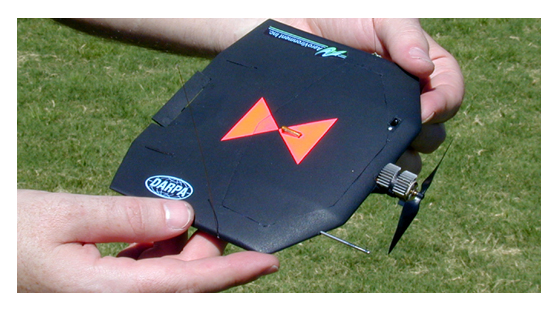
\includegraphics[width=0.5\textwidth]{images/blackwidow.eps}
	\caption{The Black Widow \cite{Grasmeyer2001} was the first operating micro aerial vehicle system, a development which was finalized in 1999 by AeroVironment for Defense Advanced Research Projects Agency (DARPA). The Black Widow can fly for up to 20 minutes and carries a very small color video camera.}
	\label{blackwidow}
\end{figure}

A micro aerial vehicle (MAV) is a subclass of the unmanned aerial vehicles (UAV). Due to their small size, the MAV can operate in numerous robotic applications, for instance, search \&  rescue, inspection and exploration. AeroVironment Black Widow \cite{Grasmeyer2001} (figure \ref{blackwidow}) is the first MAV operating in the field. The Black Widow has a fixed wing design with a single rotor. Another type of MAV is the quadcopter, which is controlled by four rotors. Quadcopters provide manoeuvrability and stability, which is suitable for indoor and urban flights. As a result of recent developments, small quadcopters with on-board stabilization have become more accessible, both in terms of price and programming interfaces. Due to this, the research regarding this platform is moving towards intelligent applications, which demand information of the surrounding environment. Nevertheless, the fast movements and the limited amount of sensor combination mean that it is still a challenge to develop navigation methods for these platforms.

\subsection{International Micro Aerial Vehicle Conference and Competitions}
The International Micro Aerial Vehicle (IMAV)\footnote{\url{http://www.imav2012.org/}} conference and competitions is an initiative that attempts to share and demonstrate new MAV technology. The competitions emphasizes on flight dynamics and autonomous flight. The IMAV consists of an indoor and outdoor competition, where these aspects are extensively tested in the various challenges. The high level of autonomy is stimulated in this competition as the rules give significantly more points to teams that operate autonomous flights. One of the problems participants have to solve is autonomous navigation through the environment. Although teams are allowed to used visual aids (ie. markers) problems in this area remain. The possible contribution of this thesis to the IMAV competition is a vision-based navigation technique for following linear-shaped objects. This navigation technique can aid autonomous flights during the challenges of the IMAV.

\subsection{Platform and Framework}
In this thesis, the Parrot AR.Drone (see
appendix \ref{PLATFORM}) and Ascending Technologies Pelican\footnote{\url{http://www.asctec.de}} are both considered as a platform. However, the Pelican had technological difficulties with the wireless connection. For this reason, the Parrot AR.Drone was chosen to perform during experiments. The AR.Drone (figure \ref{ardrone}) is a wireless controlled flying quadcopter built by the French company Parrot SA\footnote{\url{http://www.parrot.com}}. The quadcopter is made of plastic and foam and is about 30 centimetres long. It carries a horizontal and a vertical camera opening the door for the development of various visual applications. The inertial measurement unit in combination with optical flow and a ultrasound sensor provide on-board stabilization during flights allowing the quadcopter to hover in the same place. 

\begin{figure}[!ht]
	\centering
	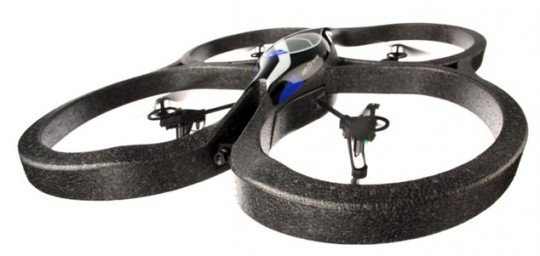
\includegraphics[width=0.5\textwidth]{images/ardrone.jpg}
	\caption{The Parrot AR.Drone is equipped with two cameras and several inertial sensors. The development is driven by commercial and research purposes. The small quadrotor allows remote observation of hazardous environments inaccessible for humans and ground robots.}
	\label{ardrone}
\end{figure}

AR.Drone SLAM \cite{Dijkshoorn2012} is a development framework for the Parrot AR.Drone developed and proposed by N. Dijkshoorn. This framework runs off-board and contains a real-time Simultaneous Localization and Mapping (SLAM) implementation based on a down-pointing camera. Therefore, it allows a MAV to know its position and movement in the environment by generating a feature map of the environment so the MAV can localize itself on this map. Furthermore, the framework facilitates control for a 3D mouse or a keyboard, and enables the generation of visual and elevation maps. Due to the framework the robot acquires more information of the environment compared to the software of the manufacturer. This information can aid the robot in navigation. In appendix \ref{PLATFORM} and \ref{FRAMEWORK} the platform and framework will be explained.

\subsection{Research questions and objectives}
\label{researchquestion}
One of the main requirements in enabling autonomous flight of MAV in GPS denied and deprived environments is the ability for navigation. One possible solution to solve this navigation problem is to use a vision-based line-following algorithm since there are various linear structures in the operating environment. There are various approaches for line-following navigation. Edge and motion detection have proven to be strong algorithms for the detection of objects \cite{Bills2011, Gerke2011}. Linear structures (ie. power lines) have a specific brightness and height, therefore, edge and motion detection are suitable algorithms. Edge detection finds sharp brightness changes in a image allowing it to find edges. Motion detection finds the disparity map, the apparent motion in a image. The disparity map shows the foreground objects brighter, denoting greater motion and lesser distance. However, these detection algorithms have their weaknesses. In order to overcome these weaknesses this thesis proposes a two stage approach, which is a common approach for object recognition \cite{Frew2004, Katrasnik2010, Gerke2011}. In the first stage edge and motion detection are combined to strengthen each other. In the second stage a Probabilistic Hough Transform (PHT) is performed to extract the line from the pre-processed image. This is a common feature extraction technique used in the field of robotics \cite{Frew2004, Zhengrong2008, Bills2011}. PHT determines a directional vector for navigation purposes and can be used to make the platform move accordingly. Based on the output of the approach the platform will navigate according to the instructions. Furthermore, this thesis is a survey for the experimental circumstances to fairly test both algorithms for a line-following task.

Therefore, the main research question is to examine how edge and motion detection can be combined to strengthen each other in a line following task. This main research question is divided up in the following sub-questions:
\begin{itemize}
\item What is the optimal configuration for the optical sensors of the platform to follow a line?
\item What are the experimental settings that demonstrate the strength and weaknesses of both algorithms clearly?
	\begin{itemize}
	\item What are the weaknesses of the algorithms?
	\item What kind of experiments show these weaknesses?
	\end{itemize}
\item What is the performance and robustness of different vision-based methods to navigation over a linear structure in a indoor environment?
\end{itemize}
In this thesis the quality of an edge and motion detection algorithm will be separately examined to determine where these can strengthen each other when combined. This in order to provide an essential component to autonomous behaviour using one camera.
\newpage
% TODO: BETER
\subsection{Outline}
Chapter \ref{RELATED_WORK} gives an overview is given over the related research regarding line-following on unmanned aerial vehicles. Chapter \ref{THEORY} gives an overview of the the theory this thesis relies on. The Computer Vision algorithms this thesis relies on are explained. The approach of this thesis is discussed in chapter \ref{ALGORITHM}. In chapter \ref{EXPERIMENTS} the experiments are illustrated and in chapter \ref{RESULTS_DISCUSSION} the results will be presented and discussed. In chapter \ref{CONCLUSION} the conclusion of this thesis will be presented and directions for future research will be proposed. Finally, additional information about the platform, framework and computer vision techniques can be found in the appendices \ref{SOURCE_CODE}, \ref{GAUSSIAN_SMOOTHING}, \ref{PLATFORM} and \ref{FRAMEWORK}.

\newpage
\section{Related Work}
\label{RELATED_WORK}
This chapter gives an overview of the related research that has been done regarding autonomous navigation for unmanned aerial vehicles. Small stable quadcopters have become affordable and research on this platform is moving towards more intelligent and autonomous applications. Various autonomous navigation methods have already been investigated in the field. First the various related autonomous applications are listed and briefly described and then a argumentation is given for the approach proposed by this thesis.

\subsection{Overview}
The following work is related to autonomous investigation for unmanned aerial vehicles:
\begin{description}
\item[Corridor and Stair Following] Corridor following is a task performed by robots for autonomous navigation in indoor environments (ie. an office). Recently, a new navigation method for the MAV \cite{Bills2011} was introduced by navigating in the indoor environment based on single image perspective cues. This is in contrast with previous approaches where a 3D model is built before planning and control. This method first classifies the type of indoor environment and then the MAV navigates through the environment using vision algorithms based on perspective cues to estimate the desired direction. The environment is detected through a confidence classifier, where estimates of the stair and corridor algorithms are used to compute the confidence values. The highest confidence value, above a threshold, is deemed as the current environment. The corridor and stair algorithm both use the the Canny edge detector and probabilistic Hough transform to acquire the line segments. The corridor algorithm then tries to determine the vanishing point in the image. The stair algorithm on the other hand tries to determine the middle of the stairs by looking at horizontal line segments of the stairs.

These vision-based methods allow MAVs to traverse corridors, stairs and corners on the basis of a small, light-weight camera, which makes them suitable for MAV with payload and power restrictions.

\item[Power Line Inspection] Power line inspection is an essential task for the maintenance of the electric grids, which is difficult due to the range of grid distributions. Over the last years rapid development has been made driven by the need for fast, accurate, safe and low-cost power line inspection \cite{Katrasnik2010}. Important requirements for power line inspection robots are to maintain position above power lines and to navigate over them, which is also the case for small aircraft. A vision-based power line following method has already been proposed \cite{Golightly2005}. This algorithm makes use of the Hough transform to detect the line segments in the image. The method makes the assumption that power lines run vertically through the screen. Therefore, the method uses the vertical line segments to adjusts its position. The main advantage of power line inspection is that the MAV can make use of the redundancy in power line design as it can follow three parallel lines. Therefore, it is easier to navigate over power lines as when one of the conductors is not detected, the MAV can adjust its position according to the other two.

Another recent approach \cite{Zhengrong2008} in power line following is to apply a Pulse-Coupled Neural Network (PCNN) to remove the background in the image. Thereafter use the Hough transform to detect the line segments and then k-means clustering is employed to discriminate power lines from other straight lines. The PCCN filter is a biological inspired approach based on the understanding of visual cortical models of small mammals. The PCCN filter is a great potential due to the low computational costs.

\item[Road-Following] Road-Following is a task performed by robots for autonomous navigation in outdoor environments. Small autonomous aircraft \cite{Frew2004} have already been able to follow a road based on real-time road detection and localization. The algorithm uses multiple vision-based method to detect the road and the lane markings. First the Bayesian Pixel Classifier, a advanced alternative of the HSV-colour filter, is applied on every pixel to see whether it belongs to the road. The classifier makes use of a database of RGB values of over 20000 pixels. Then connected-component analysis is used by labelling pixels in order to remove noise in the image and detect connected regions. After detecting the road in the image the lane markings are detected by the Bayesian pixel classification algorithm. Then a Hough transformation is applied to test multiple candidate lanes. This result in a rough discretization of the lanes. Lastly, robust line fitting, least-trimmed square, is applied to finalize the position and orientation of the center lane markings. This resulted into encouraging results, however, improvements of the algorithm can still be made.

\item[Elementary Motion Detectors] A approach presented last year during the IMAV competition by the BioMAV team \cite{Gerke2011} was to combine motion information provided by Elementary Movement Detectors (EMDs) with edge detection. EMDs are useful for UAVs due to the detection of temporal and motion effects caused by the flight of the platform. The motion information is generated by the EMD implementation \cite{Zhang2008}, which is barely dependent on differences in contrast and colour. In this approach EMDs are applied to improve the image segmentation as borders of relevant objects produce higher responses. Rotational movements of the drone will lead to edge enhancements and translational movements to larger apparent motion of objects closer to the drone. The constant self motion will provide steady and a reliable source of information. Although the EMD is useful, it rarely gives a complete picture of the environment as they rely on contrast differences. Therefore, the EMDs alone are not enough to segment the image and provide the vehicle with sufficient information. However, the EMDs provide an abundance of additional information to the traditional approach. For this reason, a combination of edge detection and motion detection is used to detect objects in the environment. EMDs filter out noise cause by the edge detection algorithm due the contrast differences in the image (see figure \ref{biomav}). From this cleaned image objects were detected by using a standard Hough transform.

\begin{figure}[!ht]
\centering
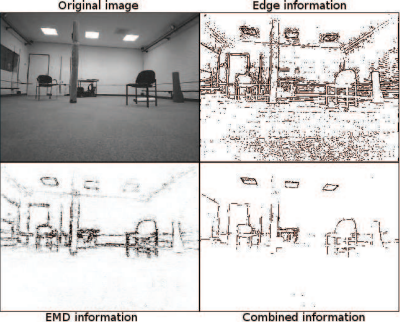
\includegraphics[width=0.5\textwidth]{images/gerke2011.png}
\caption{Example \cite{Gerke2011} of EMD for the removal of spurious edges.}
\label{biomav}
\end{figure}

\newpage

\item[Obstacle avoidance] Obstacle avoidance is a task of satisfying some control objective subject to non-collision position constraints. In obstacle avoidance the UAV requires to navigate around the obstacle to reach its objective. A recent approach uses a motion detection based algorithm to avoid obstacles in a corridor \cite{Jurriaans2011}. The approach is based on monocular stereo vision that computes the disparity map between two images. The disparity map shows the difference in motion in the environment. Obstacles that are close by have a greater motion than objects that are further away. Due to the different distances of objects the platform is able to detect and avoid them. The proposed motion detection algorithm is discussed in section \ref{MOTION_DETECTION}.
\end{description}

The above related research shows that the Hough transform is a suitable algorithm for feature extraction as nearly all approaches use a Hough Transform stage. Furthermore, edge detection and motion detection have been suitable pre-processing techniques for successful navigation \cite{Bills2011, Jurriaans2011}. In last year's IMAV competition, the combination of edge and motion detection gave promising results \cite{Gerke2011}. Given the above facts, this thesis proposes a two stage approach, where edge and motion detection will be combined to strengthen each other and the probabilistic Hough transform will be used for object recognition. The next chapter will describe the theory of the techniques.

\newpage
\section{Theory: Vision and Navigation}
\label{THEORY}
In this chapter, the basics of the theory this thesis relies on is explained. The work presented in this thesis is a continuation and extension of previous research regarding vision-based algorithms on the AR.Drone \cite{Jurriaans2011} and the Open Source Computer Vision Library (OpenCV) \cite{Bradski2008}, which provides real-time computer vision implementations.

Over the years various Computer Vision techniques have been developed to detect objects in images. One of the fundamental problems is finding the most applicable algorithm for the defined problem. In order to follow a line in flight, fast feedback from the camera is required in order for the system to adjust its trajectory. For this reason, a real-time algorithm is favourable. Furthermore, the algorithm should be able to handle movement noise caused by the motions of the flying platform. This thesis will investigate how edge and motion detection approaches can strengthen in each others weaknesses. Both approaches performance will be tested in combination with a Probabilistic Hough Line Transform \cite{Kiryati1991}, a real-time pattern recognition algorithm to detect lines.

This chapter provides an overview of theory of the Computer Vision algorithms this thesis is based on. A clear explanation will be given over the various algorithms applied in this thesis.

\subsection{Edge Detector Algorithm}
Edge detection is a tool in Computer Vision that is applied to detect identifying points in a image, where the image brightness discontinuities (see figure \ref{canny}). A line or linear structure is one of the elements in a image that causes these discontinuities. Due to the wide research over the years to edge detectors there are several implementations \cite{Ziou1998}. This thesis will focus on the Canny Edge detector as it is a suitable algorithm for edge detection. The edge detector will be applied to the images in combination with a Colour Filter, which filters out the colours not in range of the filter. An alternative that can be applied instead of the Colour Filter is the Texture Filter, which filters the texture of the infrastructure. This is also a possible approach as the platform flies at a low altitude and is able to detect infrastructure. A colour or texture filter is applied for the reason that only edges containing the same colour or texture as the line need to be detected.

% APPENDIX?
\subsubsection{Colour Filter}
To filter the colour the colour-space is converted to a different representation, namely, Hue, Saturation and Value (HSV). The HSV colour-space (in figure \ref{hsv})  is a simple transformation of the Red, Green, Blue (RGB) model and a intuitive colour-space, where separate colours can be easily filtered. The Hue stands for the visual sensation according to which an area appears to be similar to one of the perceived colors: red, yellow, green, and blue, or to a combination of two of them. Saturation is the colourfulness of a stimulus relative to its own brightness. Value is the brightness relative to the brightness of a similarly illuminated white. The three parameters have the following ranges: Hue has a range of 0$^{\circ}$-360$^{\circ}$, Saturation a range of 0-100 and Value a range 0-100.

\begin{figure}[!ht]
\centering
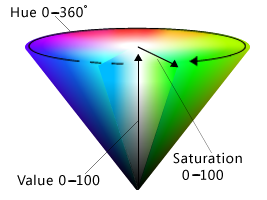
\includegraphics[width=0.3\textwidth]{images/hsv.png}
\caption{The HSV model, a cone having three parameters: Hue, Saturation and Value.}
\label{hsv}
\end{figure}

For filtering a certain colour in a image we define the ranges of the colour that has to be filtered. Every pixel is checked whether it is within this range, if so the pixel in the result image is set to 1 otherwise to 0. This result image is a binary image, where the colours in range of the colour are set to white. Colour filtering reduces the amount of noise caused by other colours in the image.

% TODO: REWRITTEN
\subsubsection{Canny Edge Detector}
The Canny Edge Detector \cite{Canny1986} is an edge detection operator that uses a multi-stage algorithm to detect edges. The aim of Canny was to develop a edge detector algorithm that is optimal for the following aspects:
\begin{description}
\item[Good detection] by marking the most real edges in the image.
\item[Good localization] by marking the edges as close to the real edge.
\item[Minimal response] by only marking edges once.
\end{description}
Calculus of variations, a mathematical technique that finds the optimal function, was applied to fulfil these requirements. The algorithm consists of the following four stages in order to reach edge detection: Noise reduction, finding the intensity gradient, non-maximum suppression and hysteresis threshold. These stages will be explained in the next sections.\\

\noindent\textbf{Noise reduction}\\
Noise reduction is applied to raw image data as the edge detector is sensitive to noise. Noise reduction can be realized by using convolution with a suitable kernel. The Canny edge detector uses a Gaussian kernel. This phenomenon is called Gaussian Smoothing (see appendix \ref{GAUSSIAN_SMOOTHING}) and filters out the small distortions so these are not detected by the edge detector. Gaussian Smoothing results into a smoothed image.\\

\noindent\textbf{Finding the intensity gradient}\\
After the noise reduction, the directional change in the intensity gradient is calculated for every pixel in the image. The intensity gradient of every pixel in the image may point in a variety of directions. Therefore, the Canny Edge Detector uses four filters to detect horizontal, vertical and diagonal edges in the smoothed image. In order to find the gradient in the image the algorithm uses a edge detection operator, which takes the first derivative of the image that results in the gradient in horizontal direction $Gx$ and vertical direction $Gy$. There are a variety of edge detection operators and the one applied in this thesis is the Sobel operator. The Sobel operator convolves (see appendix \ref{GAUSSIAN_SMOOTHING}) two $3\times3$ kernels with the image $A$ to find the horizontal $Gx$ and vertical  $Gy$ derivative, which is described in equation \ref{sobel}.
\begin{equation}
\label{sobel}
Gx =
\begin{bmatrix}
-1 & 0 & 1\\
-2 & 0 & 2\\
-1 & 0 & 1
\end{bmatrix}
* A\ \ \ \ \ 
Gy =
\begin{bmatrix}
-1 & -2 & -1\\
0 & 0 & 0\\
1 & 2 & 1
\end{bmatrix}
* A
\end{equation}
From the derivatives, the intensity gradient $G$ and direction $\Theta$ can be determined, this is illustrated in equation \ref{gradient}.
\begin{equation}
\label{gradient}
G = \sqrt{G_x^2  + G_y^2}\ \ \ \ \ 
\Theta = \arctan(\frac{G_x}{G_y})
\end{equation}
The directional angle of the intensity gradient is rounded to one of the four angles representing vertical, horizontal or the two diagonals in order to reduce computational costs of the algorithm.\\ 

\noindent\textbf{Non-maximum suppression}\\
Non-maximum suppression is the process of scanning a image along the intensity gradient direction. The pixels that are not part of the local maxima are set to zero. This suppresses all image information that is not part of the local maxima. Given the intensity gradient and direction estimates the algorithm seeks for the local maxima in the intensity gradient direction by looping over the pixels of the image. For example, if the rounded intensity gradient directional angle of the pixel is zero degrees, the pixel with a intensity gradient directional angle pointing downwards, the gradient magnitude is compared to the gradient magnitude of its left and right neighbour. If the gradient magnitude of the pixel is greater than its neighbours it will be considered a possible edge. Non-maximum suppression removes pixels that are not considered to be part of an edge. Therefore, only thin lines, candidate edges, will remain. This stage results in a binary image containing a set of possible edge points.\\

\noindent\textbf{Hysteresis thresholding}\\
The large intensity gradients are more probable to correlate to edges than small intensity gradients. For this reason, it is impossible to specify a threshold to determine whether a certain gradient is a edge or not. Therefore, the Canny Edge Detector applies another technique, namely, thresholding with hysteresis. In thresholding with hysteresis a upper and lower threshold is defined. The algorithm makes the assumption that important edges should be along continuous curves in the image, which allows the algorithm to follow a faint section of a given line and to ignore a few noisy pixels that have large gradients. Thresholding with hysteresis selects edges on the following basis:
\begin{itemize}
\item All candidates above the upper threshold will be selected as edges
\item All candidates below the lower will be refused as edges
\item All candidates between the upper and lower threshold will only be selected if it is connected to a pixel that is above the upper threshold.
\end{itemize}
This is the final step of the Canny Edge Detector and results into a binary image representing the edges in the image.

\begin{figure}[!ht]
\centering
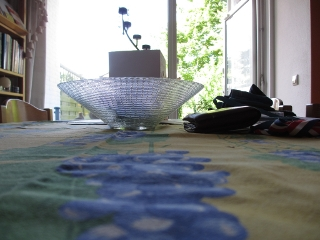
\includegraphics[width=0.3\textwidth]{images/frame0.jpg}
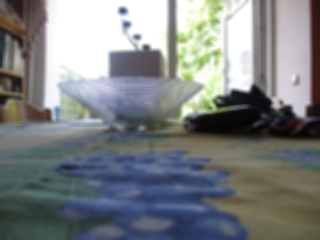
\includegraphics[width=0.3\textwidth]{images/gaussian_blur_3.png} 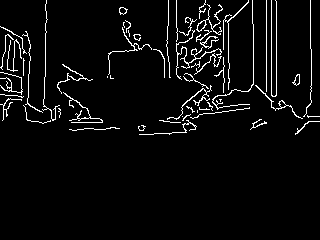
\includegraphics[width=0.3\textwidth]{images/canny.png}

\caption{Left: Original image. Middle: Smoothed image. Right: Canny Edge Detector}
\label{canny}
\end{figure}


\subsection{Motion Detection Algorithm}
\label{MOTION_DETECTION}
Motion detection is a tool in Computer Vision that is applied to detect whether an object has changed its position relative to its surroundings or the surroundings have changed relative to an object. This thesis focuses on optical motion detection from the front camera. This paper will focus on an algorithm that has been investigated for obstacle avoidance for the AR-Drone \cite{Jurriaans2011}. In this approach optical flow is calculated to determine the disparity map (see figure \ref{disparitymap}) with monocular stereo vision. The disparity map indicates whether objects in the environment are close to the camera. If a object is close to the camera it will show up brighter on the disparity map as the object has greater motion indicating lesser distance. Due to the fact that in case of this thesis the platform follows a certain linear structure in the environment it can be assumed that this structure is at a certain distance. For instance, power lines hang above the ground and will be detected closer if the platform is flying over them.
The disparity map is determined by using the resulting vectors of optical flow to calculate the fundamental matrix, which is needed to rectify images without calibration, using RANSAC. The fundamental matrix serves as the input for the Hartley algorithm that rectifies images. Finally, stereo matching is performed on the rectified images to generate a disparity map. This approach is explained in the following sections.

\subsubsection{Shi-Thomasi}
To find the optical flow in a set of images features have to be extracted from the current frame and be found in the next frame. A possibility that can provide decent features is the Shi-Tomasi algorithm \cite{Shi1994}. It tracks corners and defines a good feature in a similar approach as Harris \cite{Harris1988}, which depends on second-derivatives of image intensities. Calculating the autocorrelation of the second derivative over small windows around each point give a description of the window. According to Shi and Tomasi a good corner could be described by their eigenvalues as a good corner has eigenvalues that are greater than a minimum threshold.

As the images have a low resolution (see appendix \ref{PLATFORM}), the sub-pixel corner locations are calculated as the intensity peak is almost never centred on a pixel. By fitting a parabola on the intensity of the window and find the maximum of this parabola to determining the sub-pixel location.

\subsubsection{Optical Flow}
Optical flow is the apparent motion between an observer and the environment. A example of calculated optical flow can be seen in figure \ref{opticflow}. The algorithm tries to find the location of each pixel from one frame in the second. However, it is a challenging task to find corresponding pixels as many have the same colour and similar surrounding pixels. In order to calculate the optical flow mostly the assumption is made there is only a small movement between frames. In sparse optical flow, the most identical features are tracked across the images. Lucas-Kanade is an algorithm that makes this assumption, nonetheless it is able to track features over any distance due its pyramidal implementation.\\

\begin{figure}[!ht]
\centering
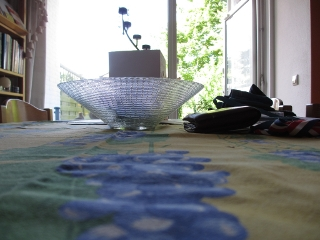
\includegraphics[width=0.3\textwidth]{images/frame0.jpg}
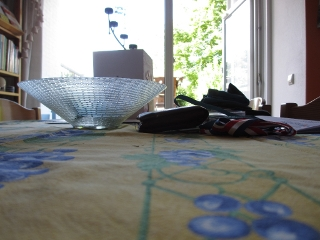
\includegraphics[width=0.3\textwidth]{images/frame1.jpg} 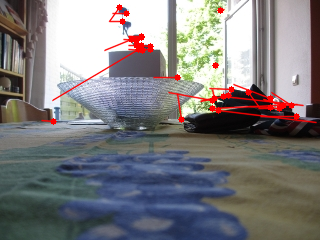
\includegraphics[width=0.3\textwidth]{images/optical_flow.png}
\caption{Left: Frame one. Middle: Frame two. Right: Optical flow.}
\label{opticflow}
\end{figure}

\noindent\textbf{Lucas-Kanade Pyramidal approach}\\
The Lucas-Kanade \cite{Bouguet2000} algorithm makes the assumption that there is only small movement in frames in order to hold equation \ref{of_equation} when small windows are taken.
\begin{equation}
\label{of_equation}
\begin{matrix}
I_x(q_1)V_x + I_y(q_1)V - y = -I_t(q_1)\\
I_x(q_2)V_x + I_y(q_2)V - y = -I_t(q_2)\\
\vdots\\
I_x(q_n)V_x + I_y(q_n)V - y = -I_t(q_n)
\end{matrix}
\end{equation}
In this equation $q_i$ stands for the pixels, $I_x(q_i)$, $I_y(q_i)$ and $I_t(q_i)$ are the partial derivatives of the image $I$ for positions $x$, $y$ and time $t$ for $q_i$. These equations can be put in matrix form as is shown in equation \ref{of_matrice}.
\begin{equation}
\label{of_matrice}
\begin{matrix}
Av = b\\\\
A = \begin{bmatrix}
I_x(q_1) & I_y(q_1)\\
I_x(q_2) & I_y(q_2)\\
\vdots & \vdots\\
I_x(q_n) & I_y(q_n)
\end{bmatrix}\\\\
v = \begin{bmatrix}
V_x\\
V_y
\end{bmatrix}\\\\
b = \begin{bmatrix}
-I_t(q_1)\\
-I_t(q_2)\\
\vdots\\
-I_t(q_n)
\end{bmatrix}

\end{matrix}
\end{equation}

This system is usually over-determined because it has more equations than unknowns. Lucas-Kanade algorithm obtains a compromise solution given by the least-square fit (see equation \ref{of_least_square}).
\begin{equation}
\label{of_least_square}
v = (A^T A)^{-1} A^T b
\end{equation}
The least square fit gives the same importance to each pixel in the window. However, practice has shown that generally it is more efficient to increase the weight of the centre pixels in the window. This is done by adding a weight matrix $W$, which is a matrix containing all the weights for each pixel. This results in equation \ref{of_weighted}.
\begin{equation}
\label{of_weighted}
v = (A^T W A)^{-1} A^T W b
\end{equation}

By gradually increasing the size of the window the optical flow over larger distances can be calculated as a least squares fit is found. A example of optical flow can be seen in figure \ref{opticflow}.

\subsubsection{Monocular Stereo Vision}
Monocular stereo vision can be used to compute a disparity map with only one camera. Stereo vision with only one camera is possible when the assumption is made that environment is static. This means that the time between the frames is not important and that the frames have to behave as if they were taken by two cameras. This assumption limits the algorithm as any moving object will violate this. To compute the disparity map the fundamental matrix has to be estimated. In stereo vision with two cameras the configuration is fixed and it is only necessary to calculate the fundamental matrix once.  However, in the case of monocular stereo vision there is only one camera and because of that it is required to find transformation between the frames for every new frame. This means that the fundamental matrix has to be found for every two frames. This is a computation complex task and difficult as for finding the fundamental matrix it is required to find points in both frames and link them together to estimate the transformation. Finding corresponding points and using them for stereo vision is known as structure from motion \cite{Varga2005}. A possible approach of finding these corresponding points is optical flow, which finds the position of a pixel in the next frame.

\subsubsection{Fundamental Matrix with RANSAC}

The fundamental matrix relates to the correspondence of each pixel location in two frames. This means that it can relate to the location of each pixel in one frame to the location of that pixel in the other frame. Together with the physical relation between two frames, the fundamental matrix can be used to calculate the essential matrix \cite{Hartley2004} that provides information about the physical coordinates. The essential matrix is a specialization of the fundamental matrix. 

In order to determine the fundamental matrix RANdom SAmple Consensus (RANSAC) is used to discriminate outliers. RANSAC takes a subset of the points and fits a model on this subset. The model is evaluated by calculating whether the remaining points are inliers or outliers. When a sufficient amount of inliers is found the model is re-determined based on all the inliers of the model. This model is then evaluated by comparing it to other models of different iterations. The model with the smallest error is kept and will be used as model. The advantage of RANSAC is that it performs well with outliers in the data.

\subsubsection{Hartley's algorithm}
After determining the fundamental matrix the images can be rectified without calibrations by using Hartley's algorithm. Hartley's approach attempts to find homographies \cite{Trucco1998} that map epipoles to infinity while minimizing the computed disparities. This achieved by matching point between the two frames, which implicitly contain the camera intrinsics. The limitation of Hartley's approach is that it does not calculate scale. This causes 3-Dimensional reconstructions to be determined by a projective transformation. This means 
that different projections of an object can appear the same to the human eye, when looking at the configuration of feature points.

Hartley first calculates the epipoles using the relations $Fe_1 = 0$ for the left epipole and $(e_r)^T F = 0$. for the right epipole. Homography $H_r$ will map the right epipole to the 2-Dimensional homogeneous point at infinity. The homography has seven contraints since scale cannot be computed. The four degrees of freedom require only three constraint to map to infinity. The four degrees have to be selected cautiously because most choices result in distorted images. 
To calculate translate $T$ that will take a selected point of interest to the origin of the right image and the rotation $R$ that will take the epipole to $(e_r)^T = ( f,0,1)$ can be calculated as shown in equation \ref{hartley}.

\begin{equation}
\label{hartley}
H_r = \begin{bmatrix}
1 & 0 & 0\\
0 & 1 & 0\\
-1/k & 0 1
\end{bmatrix}RT
\end{equation}
The homography of the left epipole can be determined by aligning the rows. Aligning by minimizing the total distance between all matching points in the frames.

\subsubsection{Stereo Matching}
After calculating the fundamental matrix and rectifying the images, the disparity map shown in figure \ref{disparitymap} can be computed between the two frames. In order to compute the disparity map, a stereo matching algorithm has to be performed. The approach taken within the research of this thesis uses a fast one-pass stereo matching algorithm \cite{Gutmann2000}. The algorithm uses sliding sums of absolute differences between pixels in the left image, while the pixels in the right image are shifted by some varying amount of pixels.


\begin{figure}[!ht]
\centering
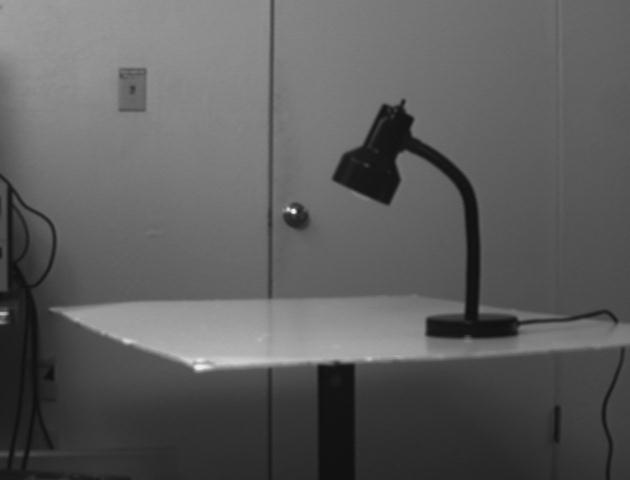
\includegraphics[width=0.3\textwidth]{images/lamp_left.jpg}
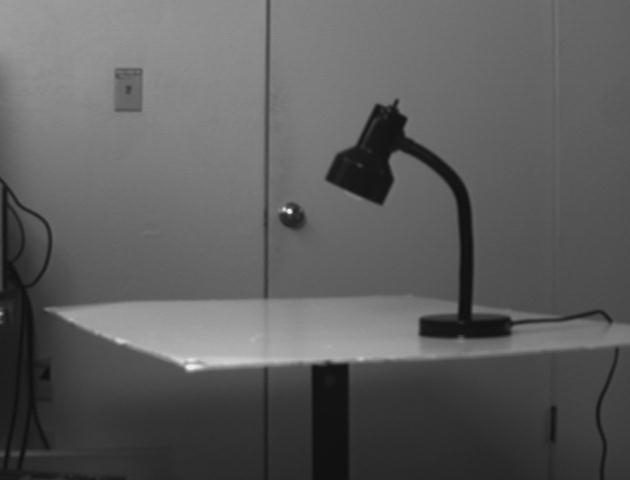
\includegraphics[width=0.3\textwidth]{images/lamp_right.jpg} 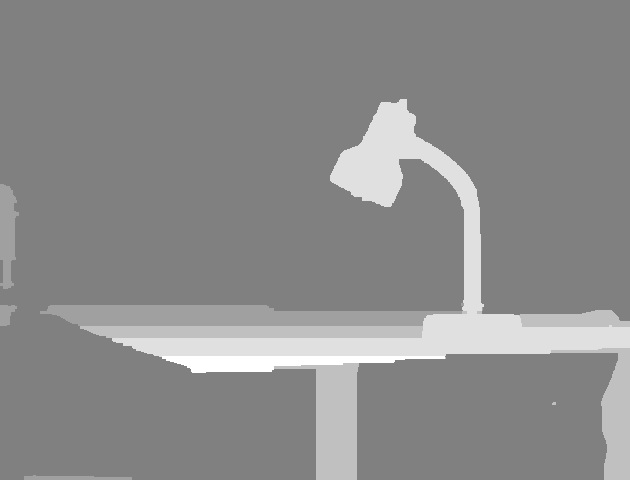
\includegraphics[width=0.3\textwidth]{images/lamp_disparity.jpg}
\caption[Disparity map]{Left: Left frame. Middle: Right frame. Right: Disparity map. Images by \href{http://vision.stanford.edu/~birch/p2p/}{Stanford University}}
\label{disparitymap}
\end{figure}

\subsection{Probabilistic Hough Transform}
The Probabilistic Hough Transform (PHT) \cite{Kiryati1991} is a feature extraction technique, which is similar to the Standard Hough Transform (SHT). PHT is applied after the pre-processing stage, which is in this case is done by an edge detector or a motion detector. Due to noise caused by the image data or pre-processing stage there may be missing points on the desired curve in the image. The goal of PHT is to address this problem by grouping edges into object candidates by performing a voting procedure over a set of parametrized image objects. In PHT lines are described in polar coordinates, distance $r$ and angle $\theta$. In the polar coordinate system $r$ is the length of the vector and $\theta$ is the angle between the origin and the vector pointing to the closest point on the line. The representation of the line in the polar coordinate system is as follows:
\begin{equation}
y = -\frac{\cos \theta}{sin \theta} x + \frac{r}{sin \theta}
\end{equation}
Every line is associated with a pair $(r,\theta)$, which is unique when $\theta \in [0, 2\pi]$ and $r \geq 0$. For every point (ie. $(x_0, y_0)$) in the image the lines that are go through are the following pairs $(r, \theta)$:
\begin{equation}
r(\theta) = x_0 \times \cos \theta + y_0 \times \sin \theta
\end{equation}
This results in a unique sinusoidal curve for every point in the $(r, \theta)$ plane. The sinusoidal curves of points that lay on the same line will have a joint intersection at the parameters for that line. All line candidates have to pass a threshold of intersections to be selected. Contrary to the SHT, the PHT takes only a subset of the points found at the pre-processing stage. For this reason, PHT is computationally faster.

\subsection{Tracking}
Tracking is the process of locating a object in multiple images. In line-following navigation it is important to receive feedback from the environment. If the visual system gives rapid feedback the system is able to react faster. For instance, when the line changes direction the platform has to adjust its angle. In order to obtain rapid visual feedback the detection method of the object should be agile.

In order to detect the line in a agile way a Region Of Interest (ROI) window is placed, once the line is found. A ROI is a selected subset of the image. The ROI is placed at the most probable place the line will appear in the next frame on the basis of the orientation of the line and motion of the platform. Since the platform is required to follow the line the ROI is frequently placed in the middle. A ROI decreases the computational costs of an algorithm as it minimizes the search window.

\newpage
\section{Algorithm}
\label{ALGORITHM}
In this chapter the various algorithms that are used for edge and motion detection for this thesis are discussed.

\subsection{Main Approach}
The main approach of this thesis for line-following navigation consists of three phases. These are the following phases:
\begin{description}
\item[Pre-processing] In the pre-processing phase, the edge and motion detection algorithms, Canny edge detector and monocular stereo vision, are applied to the image in preparation for the feature extraction phase.
\item[Feature extraction] The feature extraction phase extracts objects, in this case lines, from the pre-processed image by using a probabilistic Hough transform.
\item[Navigation] In the navigation phase, the lines found are interpreted and controls are given to the platform.
\end{description}
The system is a closed loop system, as shown in figure \ref{system_overview}, and will loop through these phases in order to keep on following the line. The approach is real-time and integrated in the AR.Drone SLAM \cite{Dijkshoorn2012} development framework (see appendix \ref{FRAMEWORK}) and can be activated by a press on the button. In this thesis the edge and motion detection were independently implemented in order to examine their strengths and weaknesses. In the following sections these phases will be described.

\begin{figure}[!ht]
\centerline{
\xymatrix{Camera \ar[rrrr]_{Frame} & & & & Pre-processing \ar[dd]_{Binary\ image}\\
& & & &\\
World \ar[uu]_{Input} & & & & Feature\ extraction \ar[dd]_{Line\ segments}\\
& & & &\\
Flight\ controller \ar[uu]_{Flying} & & & & Navigation \ar[llll]_{Controls}}
}
\caption{Schematic overview of the approach}
\label{system_overview}
\end{figure}

\subsection{Pre-processing}
There are two types of pre-processing method implemented in this thesis. In this section the implementation of the edge and motion detection, Canny edge detector and monocular stereo vision, will be described.

\subsubsection{Edge Detection}
In this thesis edge detection is implemented in the following way:
\begin{description}
\item[Colour Filter] The colour filter is applied to the image and filters for the colour of the line. The resulting binary image is combined with the result of the Canny edge detector. A colour filter was chosen as this thesis focuses on simple linear structures. However, a texture filter would also be a appropriate choice since the system flies at a low altitude, textures can easily be detected.
\item[Gaussian Smoothing] Gaussian Smoothing is applied to prepare the image for the Canny edge detector in order to remove small distortions. The resulting image is provided to the Canny Edge Detector.
\item[Canny Edge Detector] Subsequently, the Canny edge detector is applied to the image in order to find the edges indicated in a binary image. The Canny edge detector was chosen as it already was successful in previous studies regarding MAV navigation \cite{Bills2011}. For this reason, this method is suitable to be surveyed for use in combination with motion detection.
\item[Combining] The resulting images of the colour filter and Canny edge detector are combined in a image that indicates the place of the line. Combining the two techniques filters out noisy edges.
\end{description}
The result of this algorithm is a binary image containing the edges of the images. On this binary image feature extraction will be applied.
\subsubsection{Motion Detection}
In this thesis motion detection is implemented in the following way:
\begin{description}
\item[Finding features] The Shi-Tomasi algorithm \cite{Shi1994} is applied on the image in order to find good features. This for the reason that the optical flow implementation of Lucas-Kanade tracks features and this algorithm has a decent feature definition. Due to the low resolution in the images provided by the platform, the sub-pixel corner locations are calculated as the intensity peak is never centred on a pixel. The resulting features are provided for the calculation of optical flow.

\item[Optical Flow] The found features will be provided to te the Lucas-Kanade pyramidal implementation in order to find these features in the next frame. Due to the pyramidal implementation, the algorithm can find features with any distance between them. This circumvents the assumption that motion between frames is very small. This algorithm results in a set of feature pairs. The average optical flow is also computed to examine the average motion.

\item[Fundamental Matrix] Thereafter, the fundamental matrix is determined in order to rectify the images. The fundamental matrix is determined in combination with the RANSAC algorithm as the optical flow algorithm can provide noisy data. RANSAC filters out this noise and tries to find the best model for the given set of features. This results in a optimal fundamental matrix for the given features.

\item[Rectification] The fundamental matrix is required for rectifying the images without calibration. The algorithm used for this is Hartley's algorithm, which attempts to find homographies that map epipoles to infinity while minimizing the computed disparities. Resulting into rectified frames of the original frames.

\item[Stereo Matching] After determining the fundamental matrix and rectification of the original frames a fast pass stereo matching algorithm \cite{Gutmann2000} is applied to compute the disparity map. This in order to keep the implementation real-time. This step results into a disparity map indicating foreground object brighter denoting greater motion and lesser distance.

\item[Threshold] A certain threshold is taken over the disparity map in order to find the foreground object, which in this case is the line.
\end{description}
The result of this image is a binary image containing the foreground objects that have passed the threshold. On this binary image feature extraction will be applied.

\subsection{Feature Extraction}
The feature extraction method that is applied in this thesis is the probabilistic Hough transform. This method is computationally fast and deals with noise cause by the pre-processing stage. Related work (see chapter \ref{RELATED_WORK}) shows that Hough transform is a decent method for extracting features. In the case of this thesis the probabilistic form of the Hough transform\cite{Kiryati1991} is used to extract lines from the image. This form takes a only a subset of the found edges to extract features. The algorithm results into a array of lines that satisfy the criteria of the method.

\subsection{Navigation}

In order to determine the controls for the platform the found lines examined. In this thesis a simple algorithm is used that merges lines that have a similar slope and a short distance between them. The merging is done by taking the average of both lines. This reduces the amount of lines found in the image by the feature extraction method. Thereafter, the line that is the longest and has most confidence. This is measured by calculating the length of the line and counting the amount of lines this line represents. The weighted sum is taken to determine the best line found in the image.

After finding the line in the image the platform is required to navigate towards the line and follow it. This process of monitoring and controlling the movement of the vehicle. In order to navigate towards the line the trajectory has to be calculated. In order to not lose the line it is kept in the middle of the screen while navigating over it. This gives the system the following tasks:
\begin{enumerate}
\item Move towards the line in the correct orientation
\item Navigate over the line while making adjustments to keep it in the middle of the screen.
\end{enumerate}

The line that is found gives coordinates $(x_1, y_1)$ and $(x_2, y_2)$. The linear equation $y = mx + b$ can be determined from these coordinates. Given the formula of the line the adjustment can be calculated, which results in a angle $\theta$ and a translation $x$. However, flying towards the line can be done in several ways. In this thesis the platform first flies on top of the line and then corrects its orientation parallel to the line. When the platform is hovering in the correct orientation above the line it will move forward, while correcting its orientation accordingly to the line. If the platform moves to far from the line the platform will do the above step again. This is the control strategy for line-following navigation.

Furthermore, a region of interest is defined when the line is found based on the movement of the platform and location of the line. This is done to speed up the algorithm by decreasing the data it processes.
\newpage
\section{Experiments}
\label{EXPERIMENTS}
This chapter investigates the experimental settings that demonstrate the strength and weaknesses of both algorithms clearly. The proposed experiments aid to answer the previously determined research questions (see chapter \ref{researchquestion}). The various configurations, experiments and evaluation criteria will be discussed in this chapter.

\subsection{Platform}
For this thesis, the Ascending Technologies Pelican\footnote{\url{http://www.asctec.de}} and Parrot AR.Drone (see chapter \ref{PLATFORM}) were both considered for the evaluation of the vision-based algorithms. To evaluate the algorithms a stable platform with on-board stabilization was required. The Pelican has several advantages such as: on-board processing, modular design and high payload. However, the system has no indoor on-board stabilization and had technological difficulties with the wireless connection. Therefore, the Parrot AR.Drone was chosen to perform during the experiments.

\subsection{Optimal Camera Configuration}
In order to perform vision-based line-following navigation the optimal camera configuration has to be determined. In the current configuration of the AR.Drone it has a bottom and front camera. For optimal line-following navigation the camera has to point obliquely to the ground in front of the MAV. This for the reason that the platform should look ahead of itself so it can adjust itself on time. Neither the bottom or front camera provide this view as the bottom camera has a small field of view and the front camera looks to far ahead. This makes it impossible for the platform to navigate over a line as the platform cannot adapt itself to changes in time and some cases it is not even able to detect the line. Therefore, the current configuration of the cameras is not suitable for 
navigation.

\begin{figure}[!ht]
\centering
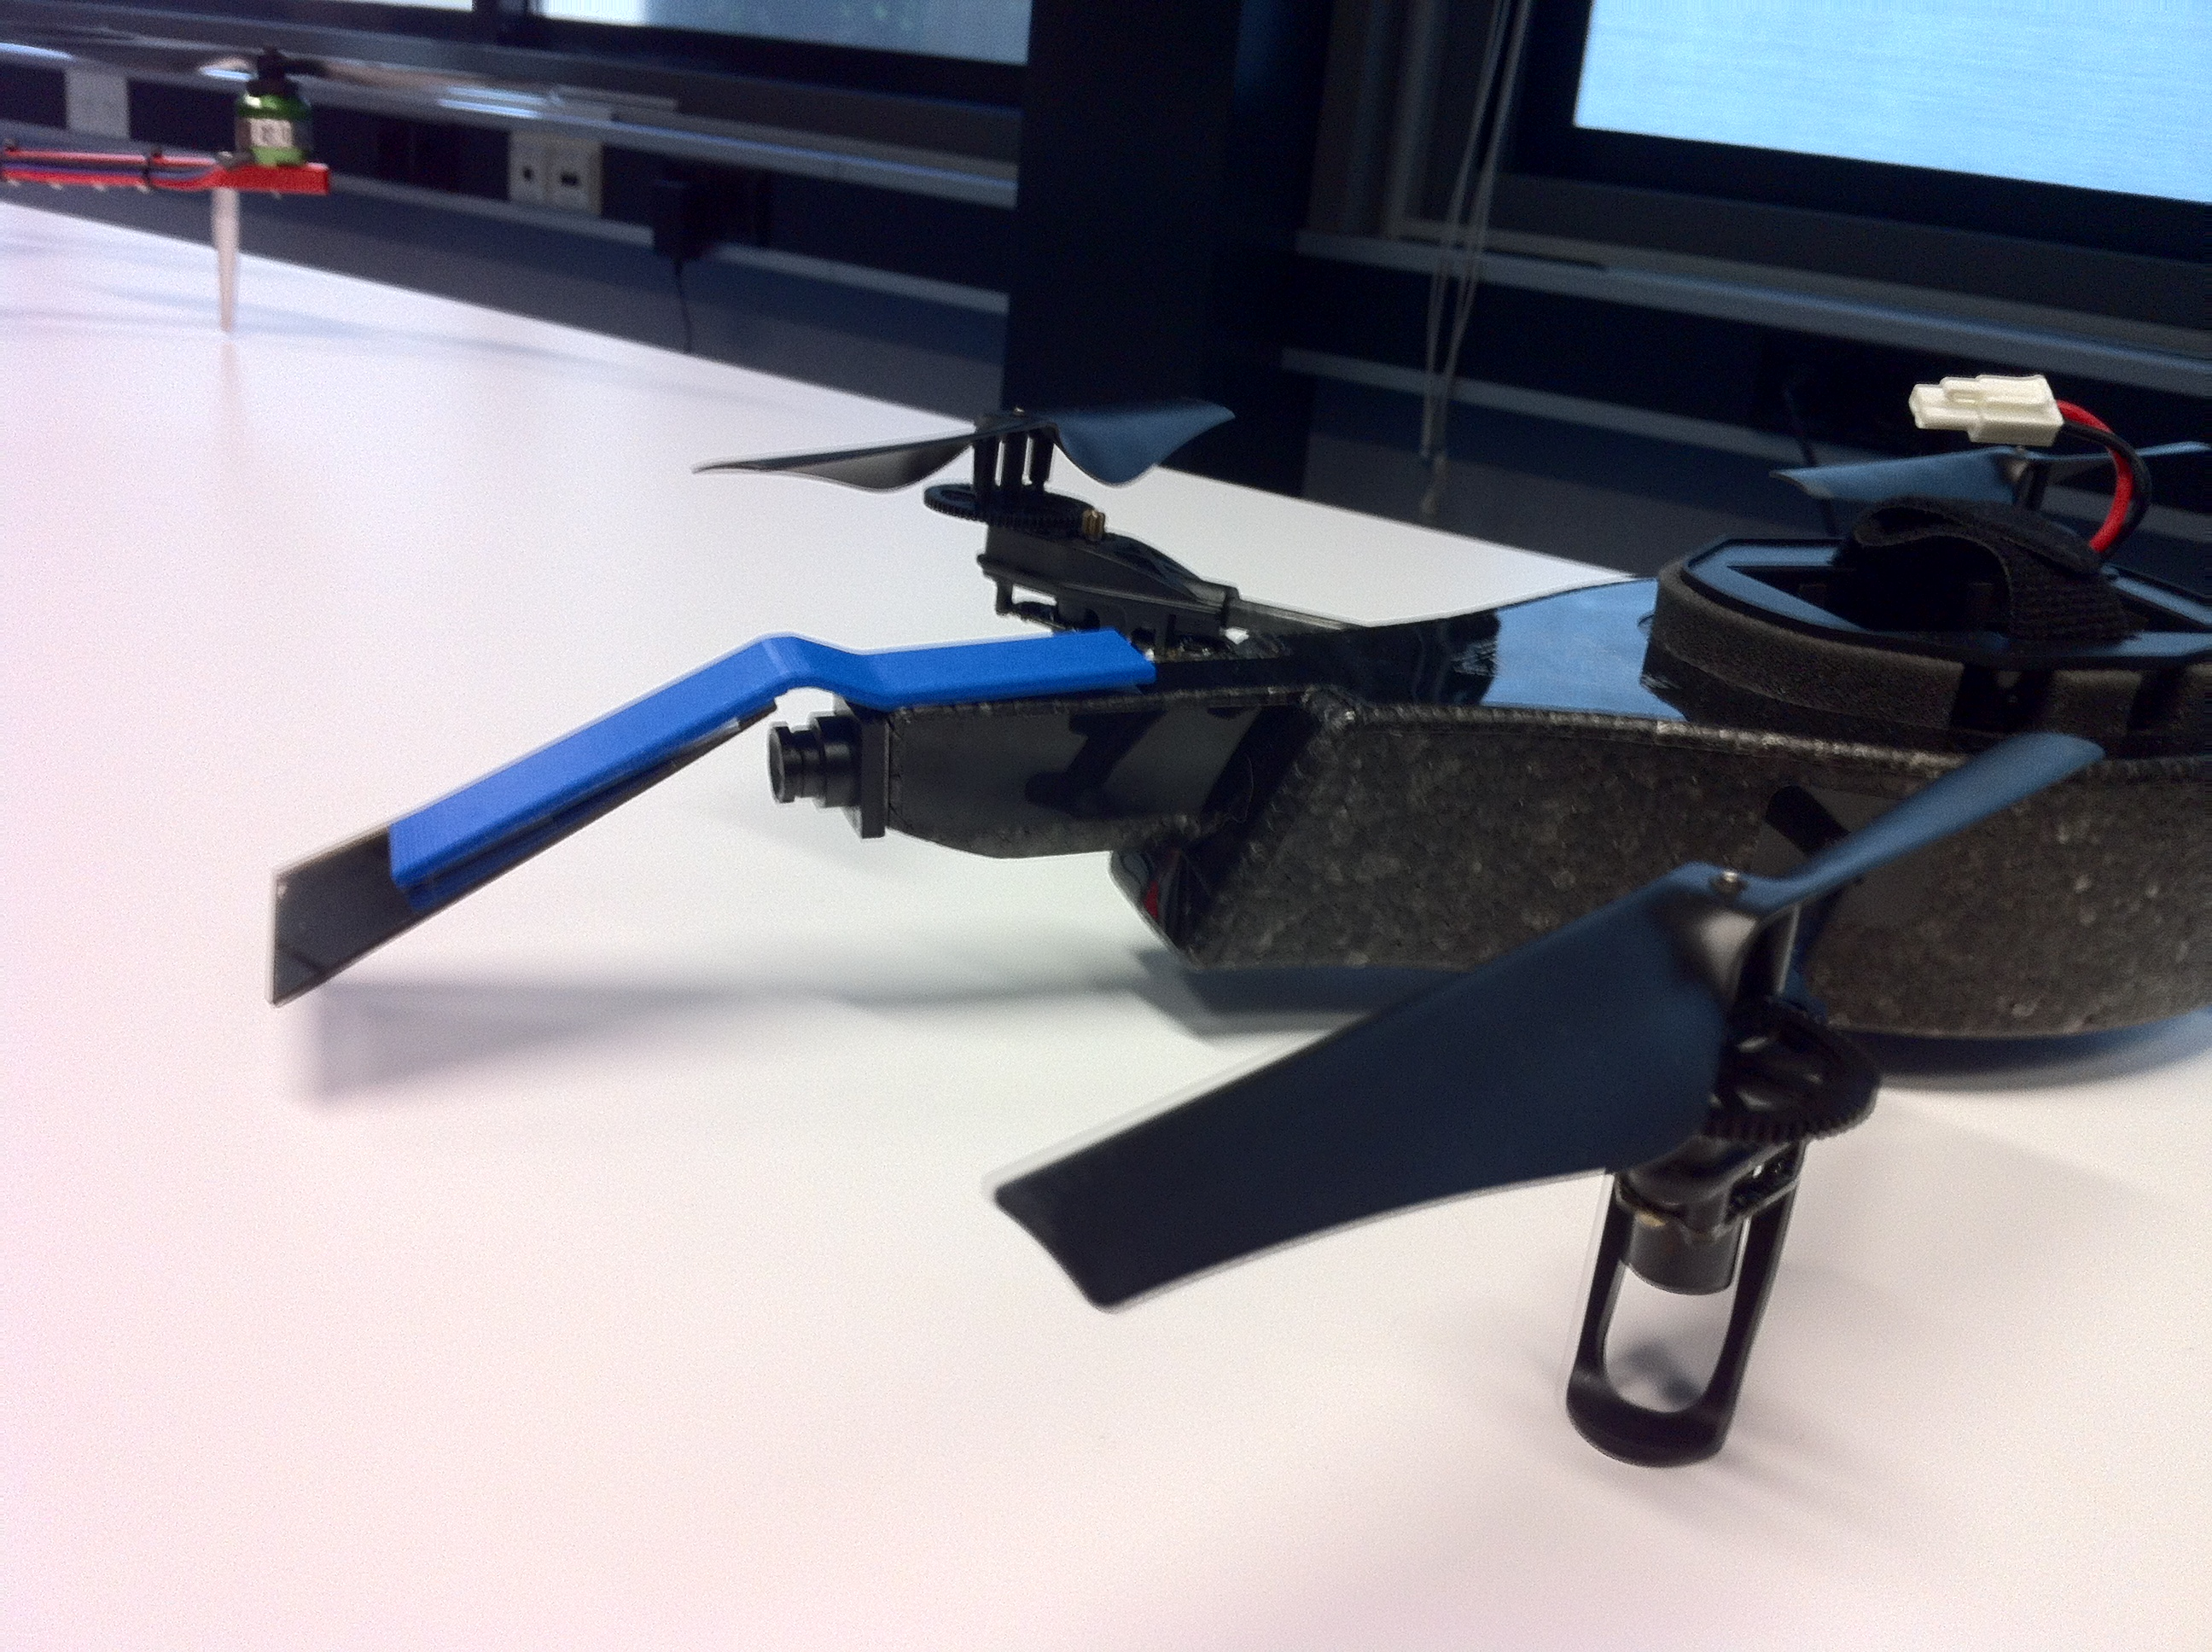
\includegraphics[width=0.3\textwidth]{images/mirror_construction.jpg}
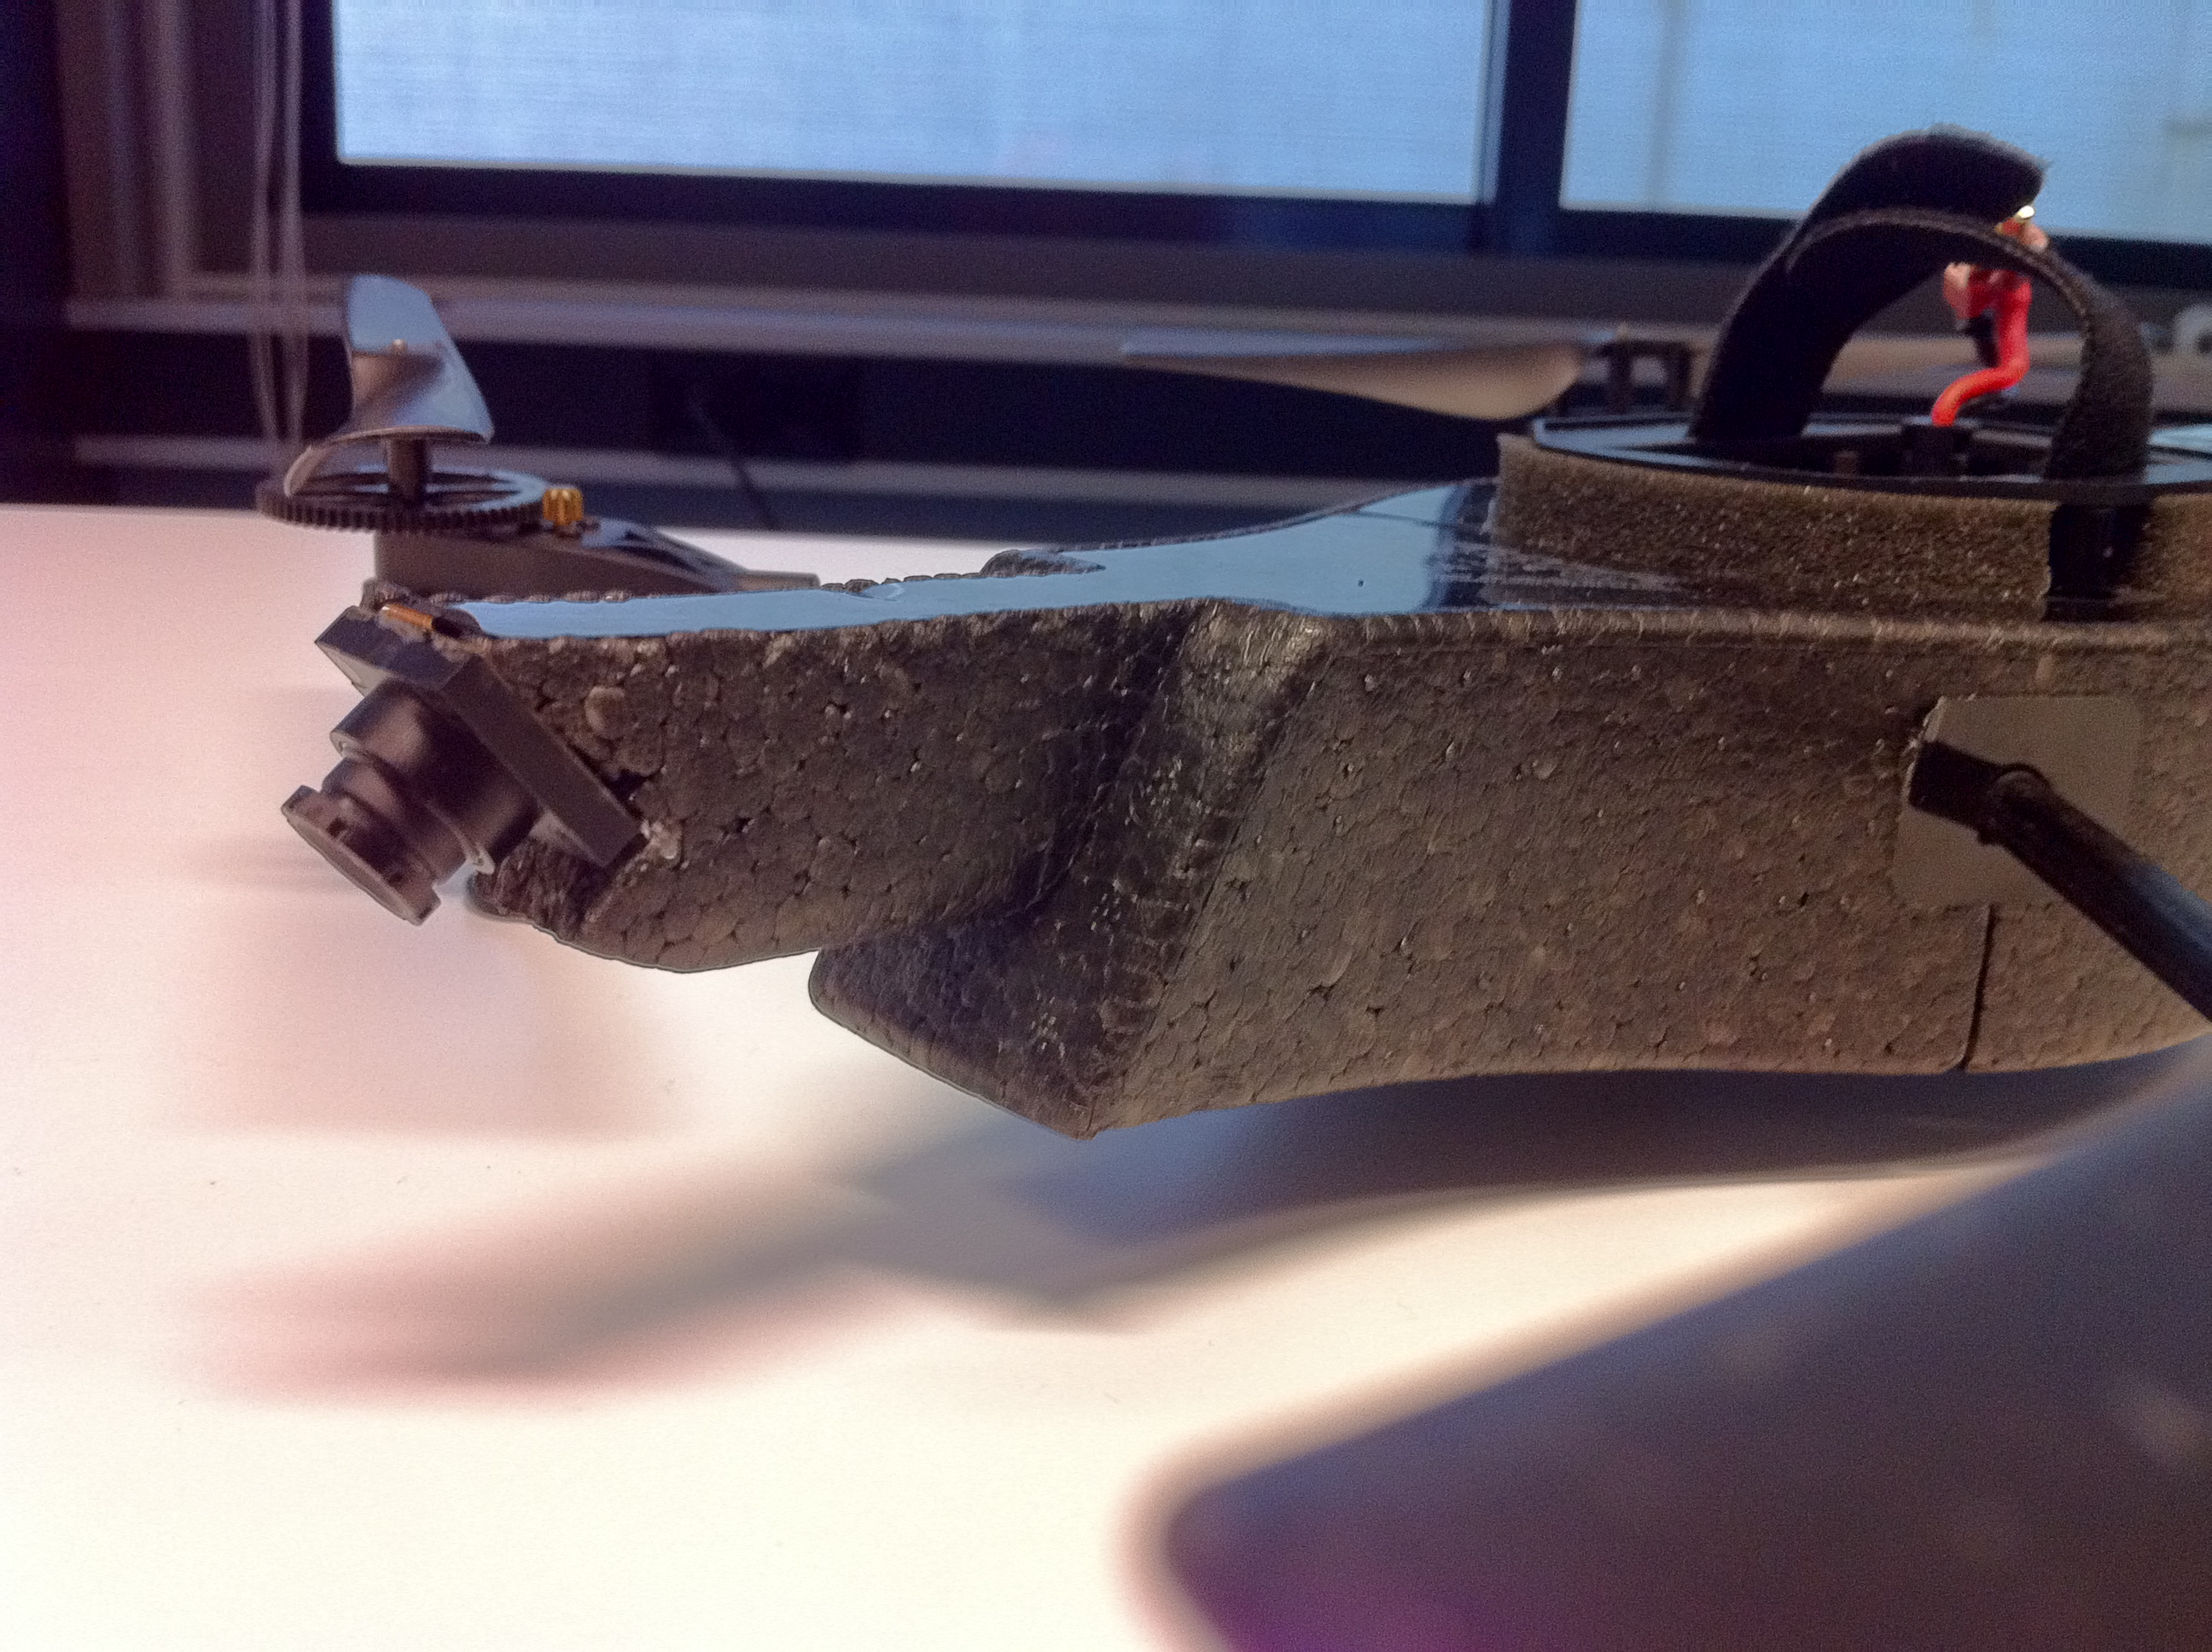
\includegraphics[width=0.3\textwidth]{images/ardrone_mod.jpg}
\caption{Possible solutions to solve the camera configuration problem, the mirror construction (left) and the modification of the AR.Drone (right)}
\label{camera_configuration}
\end{figure}

The optimal solution for the camera configuration would be the pan-tilt camera of the Pelican. The pan-tilt camera can change the angle of the camera and therefore its suitable for flying at various altitudes. Since the experiments are only indoors the platform only flies at low altitudes between 1-2 metres. Therefore, a angle of approximately 45$^{\circ}$ is considered and tested in this thesis. In order to change the angle this thesis constructed and tested the following two solutions (see figure \ref{camera_configuration}) to change the angle:
\begin{description}
\item[Mirror construction] A mirror construction that changes the view of the front camera. This construction can be placed on top of the front camera. The mirror has an angle towards the ground, which gives the camera the mirrored ahead view.
\item[Modification of AR.Drone] Modify the position of the front camera. Due to the fact that the AR.Drone is made from styrofoam its simple to modify the angle of the front camera. By cutting away styrofoam its possible to set the camera under a different angle.
\end{description}

\subsection{Experiments}
In order to investigate the strengths and weaknesses of both vision algorithms this thesis examined two type of experiments. The experiments (see figure \ref{experiments}) challenge both the algorithms. The following experiments examine the strengths and weaknesses of both algorithms:
\begin{description}
\item[Experiment One] In experiment one the weakness of the motion detection algorithm is challenged by a orange line on the ground.
\item[Experiment Two] In experiment two the edge detection algorithm is challenged by a hanging blue coloured line in the air with a blue background.
\end{description}
\begin{figure}[!ht]
\centering
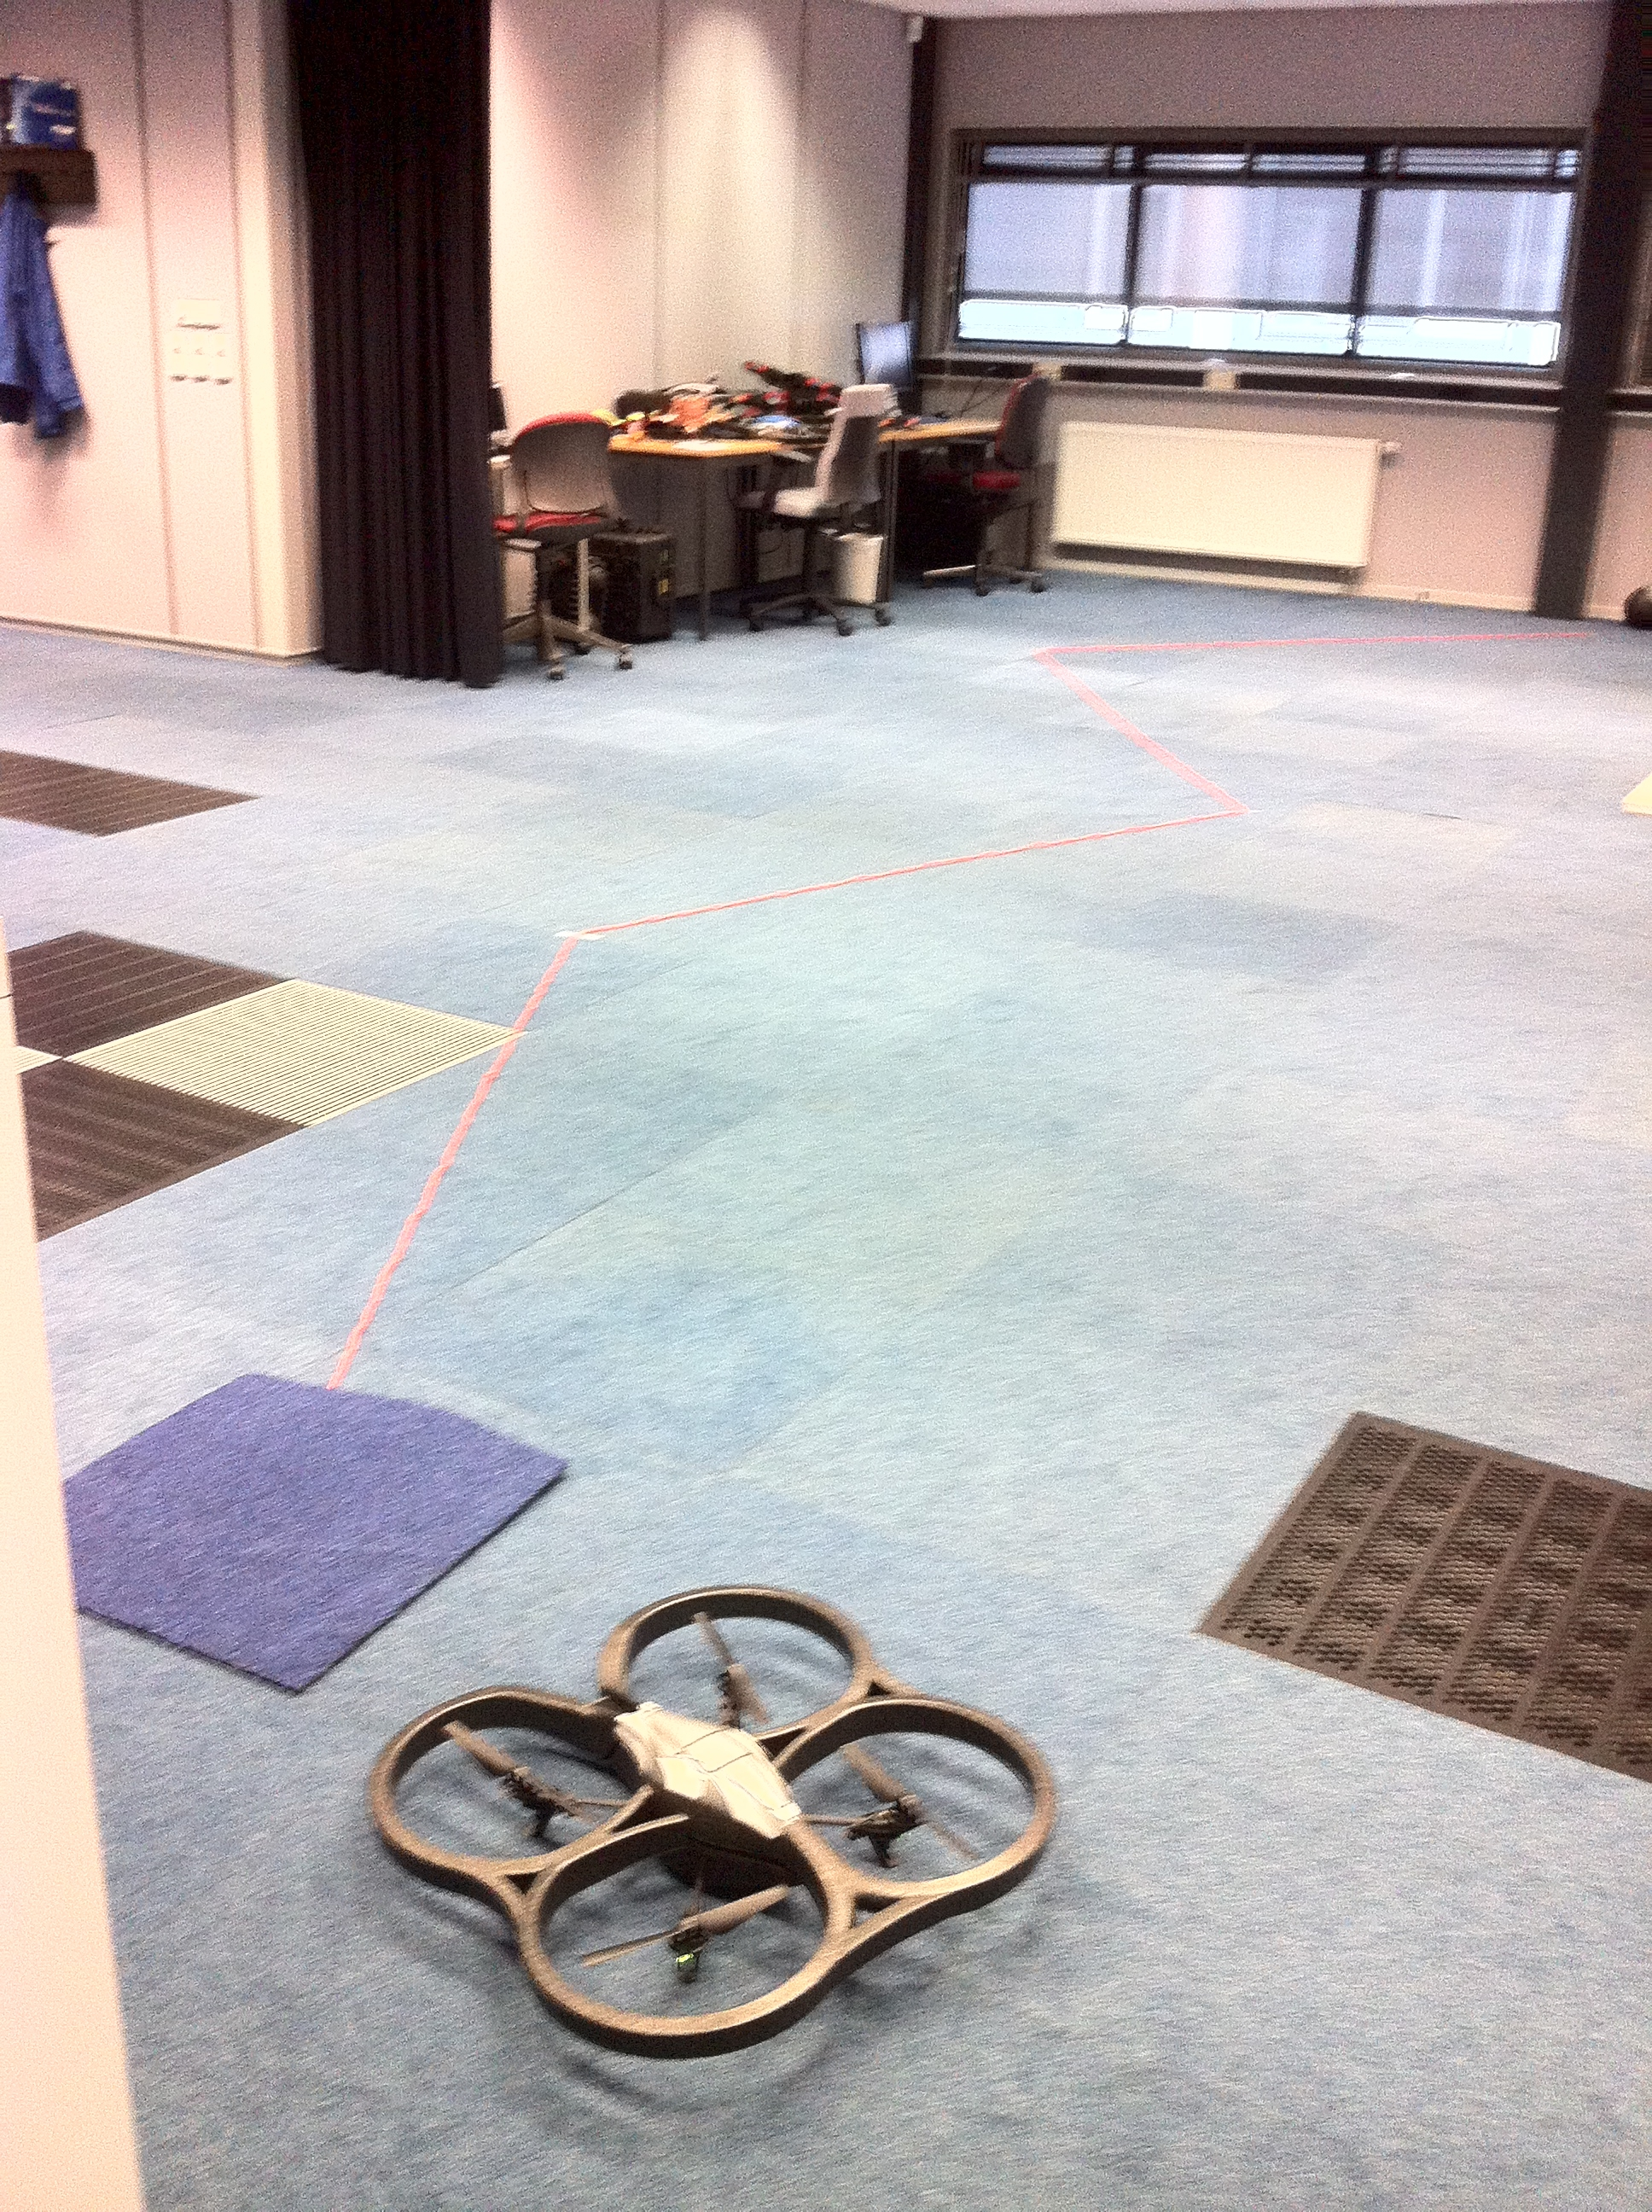
\includegraphics[width=0.3\textwidth]{images/experiment1.jpg}
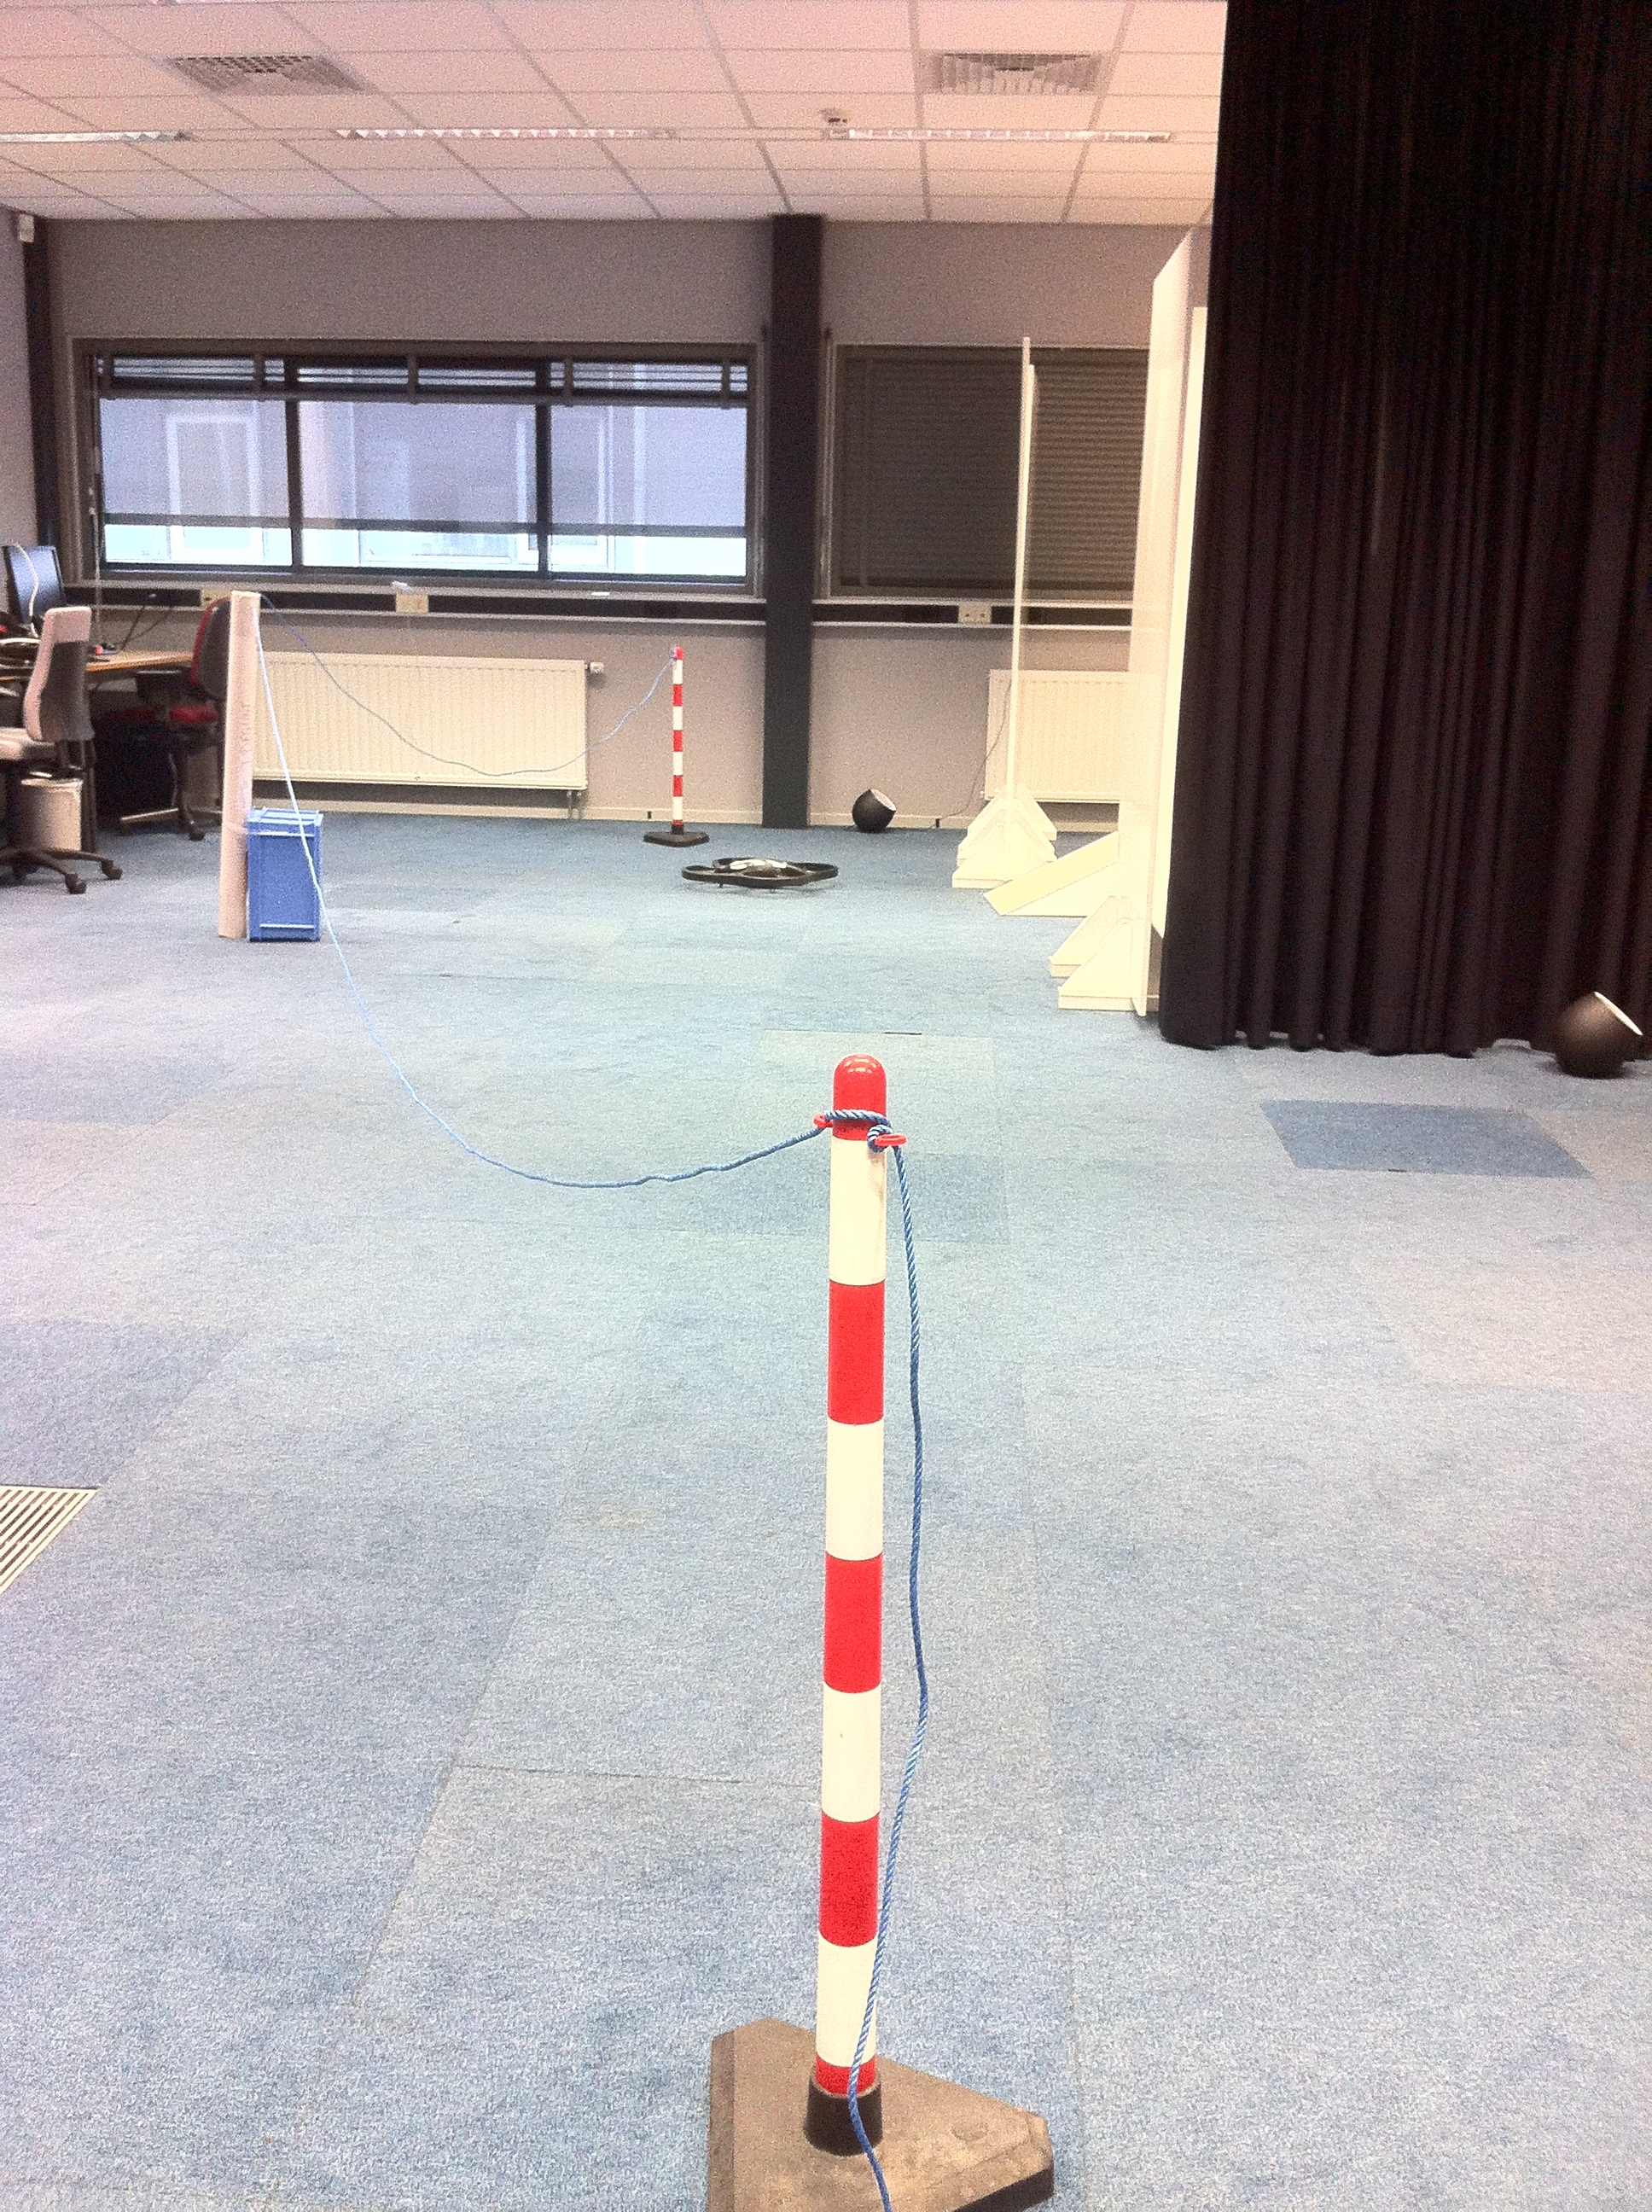
\includegraphics[width=0.3\textwidth]{images/experiment2.jpg}
\caption{On the left the setup of experiment and on the right the setup of experiment two}
\label{experiments}
\end{figure}
These experiments are challenges for both algorithms as the motion detection algorithm finds the line on the basis of distance. In contrast with the edge detection algorithm, which finds differences in brightness intensity. The strengths are also illustrated by these two experiments. In experiment one there is high contrast between the object and the background and in experiment two there is difference in height of the object and the background. These are possible situations where the two algorithms can strengthen each others weaknesses.
\newpage
\subsection{Evaluation Criteria}
To evaluate the edge and motion detection algorithms criteria are set in order to compare their performance. In this thesis the methods are evaluated based on the following two criteria:
\begin{description}
\item[Detection of lines] The number of lines the algorithm detects in the image.
\item[Direction of line] The number of lines with the correct direction.
\end{description}
Both algorithms will be evaluated on the same recorded datasets so both algorithms experience the same circumstances. The datasets are recorded, while flying the platform manually in order to prevent inaccuracies caused by navigation errors of the simple navigation method.

\newpage
\section{Results and Discussion}
\label{RESULTS_DISCUSSION}
In this chapter the results of the various experiments will be presented and discussed.

\subsection{Camera Configuration}
Before carrying out the experiments the optimal camera configuration of the platform was determined. This is done because the standard camera configuration is not suitable for line-following navigation. The following two solutions were constructed and tested in this thesis:\\

\noindent\textbf{Mirror Construction}\\
The mirror construction was designed and made on the basis of the field of view of the AR.Drone. The construction consists of a tailor made mirror that is mounted to a 3-Dimensional printed frame. The frame is placed on top of the AR.Drone as shown in figure \ref{camera_configuration}. This configuration had the following results:
\begin{description}
\item[Distorted images] The image where distorted during flight.
\item[No optimal angle] The angle of the camera towards the ground was not optimal.
\end{description}
The distorted images were caused by the vibrations of the platform during flight. The material of the frame is constructed with a thermoplastic material called Acrylonitrile butadiene styrene (ABS). The ABS material is flexible, which causes the construction to vibrate rapidly. Furthermore, the camera cannot be set to a angle of 45$^{\circ}$ without losing part of the image as the field of view of the camera is to large for this angle. Due to this the camera overlaps with the bottom camera and a smaller area is covered by the camera.\\

\noindent\textbf{Modification of AR.Drone}\\
The modification to the AR.Drone was based on the field of view of the AR.Drone. For the modification the styrofoam of the AR.Drone was cut away under a angle of 45$^{\circ}$. This gave the AR.Drone the configuration as shown in figure \ref{camera_configuration}. This configuration had the following results:
\begin{description}
\item[Sharp images] The image where clear during flight.
\item[Optimal angle] The angle of the camera towards the ground was optimal.
\end{description}
The styrofoam compensates for the vibrations of the platform. Therefore, the platform takes sharper images comparing to the mirror construction. Additionally, by modifying the AR.Drone the camera can be put at any angle. However, the modification cannot be undone, which is a disadvantage.

\subsection{Edge Detection}
After determining the camera configuration, the edge detection algorithm was tested on several images. The colour filter and the Canny edge detector in combination with a Gaussian blur were applied over these images. The result of the colour filter and the Canny edge detector were combined in a image, which was provided to the probabilistic Hough transform. This resulted into an array of possible line segments. The best line was determined and indicated on the image. In figure \ref{edge_detection_results} typical results can be seen of this algorithm. 

These results look promising, however, the line is detected simply as there are high intensity differences in the image. The combination of the colour filter seems to work well for filtering out the noisy edges. Note that the probabilistic Hough transform is performing well on the pre-processed images.
\begin{figure}[!ht]
\centering
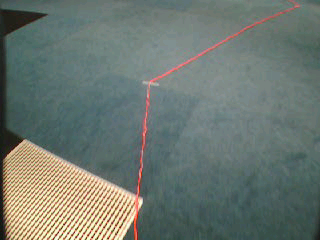
\includegraphics[width=0.3\textwidth]{images/canny_image.png}
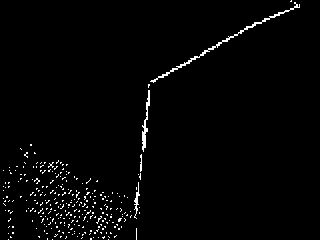
\includegraphics[width=0.3\textwidth]{images/canny_image_filter.png}
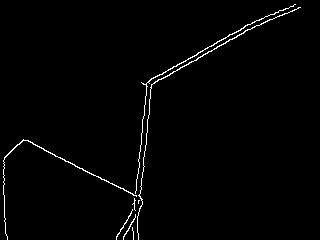
\includegraphics[width=0.3\textwidth]{images/canny_detector.png}\\
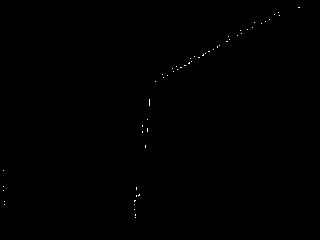
\includegraphics[width=0.3\textwidth]{images/canny_combine.png}
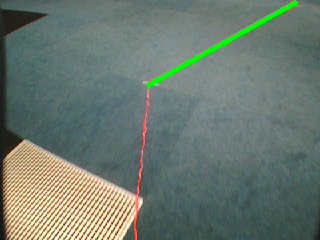
\includegraphics[width=0.3\textwidth]{images/canny_PHT.png}
\caption{First row: Original Image, Colour Filter and Canny Edge Detector. Second row: Combined Image and the Probabilistic Hough Transform result.}
\label{edge_detection_results}
\end{figure}

\subsection{Motion Detection}
The motion detection algorithm was also tested before being evaluated. The optical flow was calculated on the basis of the features that were found by the method of Shi-Tomasi \cite{Shi1994}. From the corresponding points the fundamental matrix was determined using RANSAC to discriminate the outliers. The fundamental matrix served as input for Hartley's Algorithm that rectified the images. These images were used to compute the disparity map, which was thresholded to find the closest foreground object. The resulting image served as input for the probabilistic Hough transform, which extracts the lines from the provided images. The best line was determined and indicated. In figure \ref{motion_detection_results} a sample result of this algorithm is shown.

The result of the motion detection algorithm looks reasonable. Nevertheless, this was tested on a ideal situation where the line is hanging close to the platform. It seems that the algorithm sometimes is unable to detect the line due to the lack of motion between the frames. This is in line with the theory behind Monocular Stereo Vision as then its hard to see any motion.
\begin{figure}[!ht]
\centering
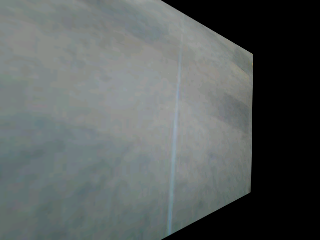
\includegraphics[width=0.3\textwidth]{images/stereo_left.png}
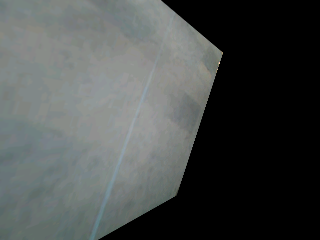
\includegraphics[width=0.3\textwidth]{images/stereo_right.png}
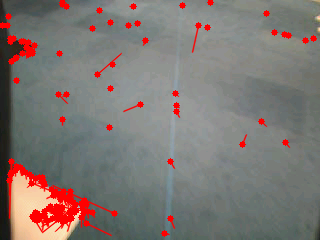
\includegraphics[width=0.3\textwidth]{images/stereo_optical_flow.png}
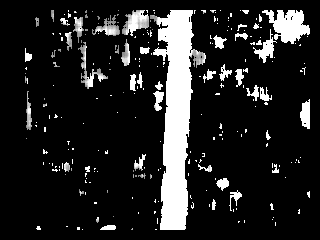
\includegraphics[width=0.3\textwidth]{images/stereo_disparity.png}
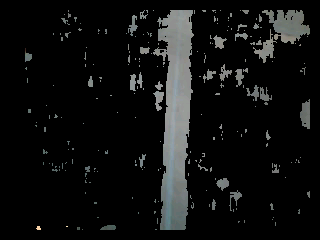
\includegraphics[width=0.3\textwidth]{images/stereo_disparity_cut.png}
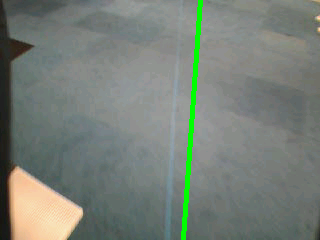
\includegraphics[width=0.3\textwidth]{images/stereo_PHT.png}
\caption{First row: Left Image, Right Image and Optical Flow. Second row: Disparity Map, Disparity Map on Image and the Probabilistic Hough Transform result.}
\label{motion_detection_results}
\end{figure}

\subsection{Experiment One}
In experiment one the platform was acquired to fly over a orange line on the ground. The edge and motion detection were both evaluated on the same dataset. The vision algorithms were evaluated on the amount of times a line was detected and whether the detected line had the correct direction. This gave the following results:\\

\noindent\textbf{Edge Detection}\\
\begin{tabular}{| l | l | l |}
\hline
\textbf{Performance} & True & False\\
\hline
Detected  & 528 (97.8\%) & 12 (2.2\%)\\
\hline
Direction & 503 (93.1\%) & 37 (6.9\%) \\
\hline
\end{tabular}
\newpage
\noindent\textbf{Motion Detection}\\
\begin{tabular}{| l | l | l |}
\hline
\textbf{Performance} & True & False\\
\hline
Detected  & 53 (9.8\%) & 487 (90.2\%)\\
\hline
Direction & 37 (6.9\%) & 503 (93.1\%) \\
\hline
\end{tabular}\\

These results evidently show that this experiment is a weakness of the Motion Detection algorithm. All the features in the image move in the same motion, therefore, the algorithm only detects background. This results in a disparity map without any depth. On the other hand the performance of the edge detection algorithm is satisfying. The results obviously show the strength of edge detection and the weakness of motion detection. Therefore, edge detection can strengthen motion detection.

\subsection{Experiment Two}
In experiment two the platform was acquired to fly over a hanging blue coloured line with a blue background. The edge and motion detection were both evaluated on the same dataset. The vision algorithms were evaluated on the amount of times a line was detected and whether the detected line had the correct direction. This gave the following results:\\

\noindent\textbf{Edge Detection}\\
\begin{tabular}{| l | l | l |}
\hline
\textbf{Performance} & True & False\\
\hline
Detected  & 69 (29.0\%) & 169 (71.0\%)\\
\hline
Direction & 58 (24.4\%) & 180 (85.6\%) \\
\hline
\end{tabular}\\

\noindent\textbf{Motion Detection}\\
\begin{tabular}{| l | l | l |}
\hline
\textbf{Performance} & True & False\\
\hline
Detected  & 96 (40.3\%) & 142 (59.7\%)\\
\hline
Direction & 87 (36.6\%) & 137 (63.4\%) \\
\hline
\end{tabular}\\

These results show that motion detection is performing better than edge detection. However, the motion detection algorithm is not as robust as edge detection in experiment one. This is because between some frames in the dataset was not enough distance making the method unable to detect motion in the image. This is causing the weak performance of the algorithm as it was able to detect continuously the line. Furthermore, the results show that low gradient intensity differences are hardly detected by an edge detector. Due to the fact the motion detection algorithm is able to detect the line when there is enough motion it can strengthen edge detection.\\

\noindent All in all, the above results show the weaknesses and strengths of the edge and motion detection algorithms. Edge detection is good at detecting differences in gradient intensity of the image. On the other hand motion detection is good at detecting foreground objects assuming that there is enough motions in between the frames. The results show that combining the two would strengthen others weaknesses. Therefore, fusing these two algorithms is a suitable approach for the pre-processing stage of a probabilistic Hough transform.



\newpage
\section{Conclusion}
\label{CONCLUSION}
In this thesis a two stage approach is proposed that combines edge and motion detection with a probabilistic Hough transform. This for the reason that both pre-processing techniques strengthen each others weaknesses. Where edge detection finds sharp brightness changes, motion detection finds the foreground objects. The results of the experiments show the strengths and weaknesses of both algorithms. The results also show that there is no optimal vision-based approach. Therefore, fusing algorithms will make vision-based methods more robust.

The optimal configuration of the camera for the line-following task was determined in this thesis. The front camera was set to a angle of 45$^{\circ}$ by modifying the AR.Drone. This was the best and most stable solution in order to solve the camera configuration problem. A mirror construction was also examined. However, this was unstable in the sense that the mirror was vibrating during flights. Additionally, this construction could not obtain the optimal angle.

Two experiments where designed to show the strengths and weaknesses of the edge and motion detectors. In the first experiment, motion detection was challenged and in the second experiment, edge detection. The results of the experiments show that these algorithms strengthen each others weaknesses.

The performance and robustness of both vision-based algorithms showed promising results and can be used for a line-following task. However, when edge and motion detection are combined this can lead to even more robust vision-based algorithms.

Conclusively, this thesis examined the strengths and weaknesses of two different kind of pre-processing techniques, namely, edge and motion detection. From this examination can be concluded that indeed edge and motion detectors can strengthen each other. Therefore, this thesis recommends a combination of these two algorithms to autonomously follow linear shaped structures in a landscape.

\newpage
\section{Future Research}
For a MAV to be able to navigate autonomously in a indoor or urban environment it is necessary to use a navigation method as proposed in this thesis. For navigation accurate controls are required, which are provided by the visual system. The controls provided by the visual system should be accurate as it is not affordable to crash. The visual system of the MAV can be more robust by combining the strengths of these vision-based algorithms. Also other methods can aid the robustness of a vision-based algorithms:
\begin{description}
\item[Localization] Probabilistic methods such as the Kalman Filter \cite{Welch1995} can aid keeping track of the location of the line. A Kalman Filter is an algorithm which uses a series of measurements observed over time, containing noise, produces estimates of unknown variables that tend to be more precise than those that would be based on a single measurement.
\item[Navigation Method] The navigation method should be improved so it can handle multiple lines. A smarter navigation module leads to more intelligent applications.
\item[Evaluation Criteria] More evaluation criteria should be examined to determine whether a vision-based algorithm is successful.
\item[Environments] The various vision-based algorithms should be tested in a wide range of environments to determine their robustness.
\item[Algorithms] More vision-based algorithms have to be investigated for their strength and weakness in order to successfully combine them.
\end{description}
All of the above points would extend the knowledge about vision-based algorithms on the MAV.

\newpage
\begin{appendices}
\section{Source code}
\label{SOURCE_CODE}
All the source code is available at the GitHub repository:\\ \url{https://github.com/camielv/ThesisVerschoor}.\\
The recorded datasets are available here:\\
\url{https://github.com/camielv/ThesisVerschoor/Datasets}\\
A research log can be found here:\\
\url{http://camielv.nl/thesis}\\
The following videos show the results of the algorithms:\\
Edge detection on dataset: \url{http://youtu.be/GqdAJ3AUrmg}\\
Motion detection on dataset: \url{http://youtu.be/cSdcYHPiah4}\\
Line-following navigation: \url{http://youtu.be/MmxhRnjHIv4}

\newpage
\section{Gaussian Smoothing}
\label{GAUSSIAN_SMOOTHING}
% TODO: REWRITTEN
This chapter provides a explanation for Gaussian Smoothing. The convolution technique is discussed first and then the Gaussian kernel of convolution is explained.\\

\noindent\textbf{Convolution}\\
Convolution is a mathematical way to combine two functions. The mathematical definition of convolution for the two scalar functions $f(x)$ and $g(x)$ is:
\begin{equation*}
h(x) = \int_{-\infty}^\infty f(u)g(x - u)du
\end{equation*}

The integral expresses the amount of overlap of function $g(x)$
due the shift over the other function $f(x)$. This causes one function to blend with the other. The convolution operator contains the following algebraic properties: commutativity, associativity and distributivity. Convolution is commonly applied in computer vision in order to detect edges in a image. In figure \ref{gaussianblur} a example of a convolution with the Gaussian Kernel is illustrated.
\begin{figure}[!ht]
\centering
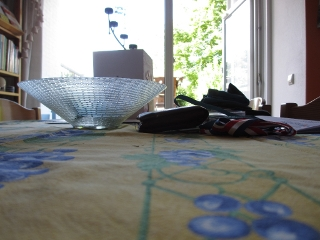
\includegraphics[width=0.3\textwidth]{images/frame1.jpg}
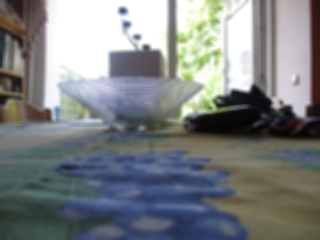
\includegraphics[width=0.3\textwidth]{images/gaussian_blur_3.png}

\includegraphics[width=0.3\textwidth]{images/gaussian_blur_11.png}
\caption[Gaussian Blur]{Left: original. Middle and right: Gaussian Blur of 3 and 11 pixels.}
\label{gaussianblur}
\end{figure}

\noindent\textbf{Gaussian Kernel}\\
The most suitable kernel for an optimal convolution is the Gaussian function due to the smoothing, derivatives and separability. The Gaussian function has the best smoothing properties as it has existing derivatives to any order at every point. Due to this every function can be smoothed as the derivative is always non-zero. In image processing the intensity is smooth smoothed intensity of a image this can be done by convolving the original image with the derivative of the Gaussian function. Gaussian Smoothing is the result of blurring an image by a Gaussian Function. Smoothing is applied to reduce noise and detail in the image. Gaussian smoothing is a well know technique mostly used in computer vision algorithms as a pre-processing technique in order to enhance image structures at different scales. Gaussian Smoothing is the same as convolving the image with a Gaussian function. The 2D Gaussian smoothing function is represented by the following equation:
\begin{equation*}
G(x,y) = \frac{1}{2\pi\sigma^2}e^{\frac{x^2 + y^2}{2\sigma^2}}
\end{equation*}

\newpage

\section{Platform}
\label{PLATFORM}
One of the basic steps for the development and testing of intelligent applications in robotics is to find an applicable robot platform for the defined problem. A common choice for a Unmanned Aerial Vehicle (UAV) is to use a quadcopter. The small size and manoeuvrability allows both indoor and outdoor flights. Moreover, quadcopters have a simple design due to the fact that they do not require mechanical connections to vary the pitch angle of rotor blade.
As a result of technological developments in aerospace engineering of UAV's, a small quadcopter with on-board stabilization have become more accessible, both in terms of price and programming interfaces. Because of this, research regarding this platform is moving towards more intelligent applications, which demand information of the surrounding environment. The specific platform selected for the experiments in this research is the Parrot AR.Drone quadcopter. The advantages of this platform are its on-board stabilization, lightweight and the affordable price of the platform. The AR.Drone is carrying a front and bottom camera that provide live video streaming through a Wifi data link.  The platform is controlled via the same data link, which allows the user to send commands and receive data of the platform.
In this chapter, the AR.Drone platform is described. The operational part of te platform is discussed, the hardware the platform contains is described and the software development kit is briefly described.

\subsection{Quadcopter}
A quadcopter consists of four rotors that are attached to a main frame, which commonly has a cross-shaped form (see figure \ref{quadcopter}). Every rotor produces thrust $T$ and torque $\tau$ over the center of rotation, whereas it also produces drag force $D_b$ in the opposite direction of flight. Thrust $T$ is the force that is generated by increasing and decreasing acceleration the mass in one direction. The acceleration of the mass will result in a force of equal magnitude but in the opposite direction of the platform. Torque $\tau$ is the force that rotates an object around its axis. Drag $D_b$ is the force that is in opposite direction to the motion of the aircraft through air. This force is inclined on the velocity of the quadcopter and de-acceleration will take place if insufficient thrust is generated. The rotors together should generate sufficient thrust to stay airborne during flights.

\begin{figure}[!ht]
	\centering
	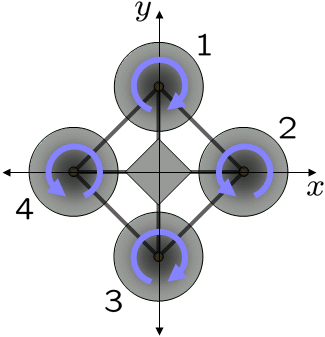
\includegraphics[width=0.25\textwidth]{images/quadcopter.png}
	\caption{Diagram of the reaction torgues on each motor of the quadcopter, due to the rotors. Rotors one and three are spinning clockwise, whereas rotor two and four spin counter-clockwise, causing opposing force for control}
	\label{quadcopter}
\end{figure}

In order to fly, the quadcopter relies on differences in thrust and torque. Pitch, roll and yaw (see figure \ref{plane}) is the naming of flight dynamics to indicate the rotation angles in three dimension of the center mass of the quadcopter. The opposing rotor pairs (pair 1, 3 and pair 2, 4) turn in the same direction. One of the pairs is turning clockwise, while the other pair turns counter-clockwise. This causes the platform to have no angular acceleration, when all rotor pairs have the same angular acceleration. Alternating the angular speed of the rotor pairs will cause angular acceleration about the yaw.

\begin{figure}[!ht]
	\centering
	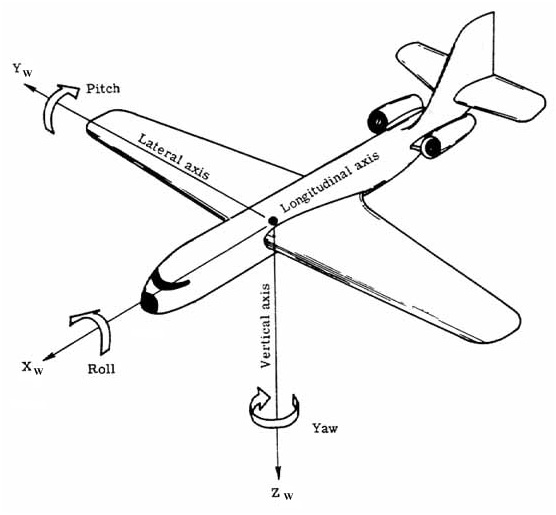
\includegraphics[width=0.5\textwidth]{images/plane.jpg}
	\caption[plane]{Diagram of pitch, roll and yaw rotations on an aerial vehicle. By \href{http://mtp.mjmahoney.net/www/notes/pointing/pointing.html}{M. J. Mahoney}}
	\label{plane}
\end{figure}

Vertical movements are accomplished by changing the thrust from each rotor alike, which is causing the resulting thrust to change and the differential torque to remain zero. Moreover, when the thrust is kept constant the vertical velocity remains the same. Horizontal movements are caused by changing the pitch and roll angle. Angular accelerations over the pitch and roll angles can be generated independently. Each pair of opposing rotors controls either pitch or roll rotation of the platform. A torque balance is kept for yaw stability during differential torque over the roll and pitch by increasing the speed of one rotor, while decreasing the speed of the opposing rotor.

\subsection{Hardware}
The AR.Drone is a remote-controlled quadcopter developed by the French company Parrot SA for consumer use. The main frame is made of carbon fibre and high resistance plastic. The AR.Drone has an indoor and outdoor hull, which is used for protection of the system. The rotors are powered by motors, whom are connected to a lithium battery allowing the system to fly approximately ten minutes.

The AR.Drone has a sensor suite containing an six degrees of freedom Inertial Measurement Unit (IMU), a bottom camera and a ultrasound altimeter used for automatic stabilization. The IMU consists of a three axis accelerometer, a two axis roll and pitch gyrometer and a single axis yaw gyrometer. The IMU reports on the system its velocity, orientation and gravitational forces. The ultrasound altimeter measure the altitude of the system and in combination with the bottom camera it calculates the optical flow of the system. All the above sensors contribute to the on-board stabilization module of the quadcopter, which allows the quadcopter to hover in one place.

\subsubsection{AR.Drone 1.0}
The AR.Drone has an on-board computer running a custom Linux operating system. A mini-USB connector is included on the system for software maintenance and additional external sensors (e.g. GPS sensor). The integrated wireless card provides network access for external devices that control the vehicle. The onboard software is proprietary of the manufacturer, however, an application programming interface is provided.

The horizontal camera has approximately 75$^{\circ}$ x 60$^{\circ}$ field of view and provides 640 x 480 pixel color images. The bottom camera provides color images with 176 x 144 pixels and its field of view is approximately 45$^{\circ}$ x 35$^{\circ}$ \cite{Krajnik2011}.

\subsubsection{AR.Drone 2.0}
Recently, Parrot brought a new platform on the market, the AR.Drone 2.0. This new platform has a similar configuration as its predecessor, however, most of the components have been improved. The new on-board technology gives better stabilization and more precise sensor measurement comparing to their previous platform. The AR.Drone two carries a horizontal camera with a resolution of 1280 x 720 pixels and the vertical camera a resolution of 320 x 240 pixels. Furthermore, it has an electronic compass. These improvements aid intelligent vision-based applications as more detailed images give more information about the environment.

\subsection{Software Development Kit}
Parrot created a open source Software Development Kit (SDK) providing developers the opportunity to create intelligent applications for their platform. The SDK comes with source code, multiplatform examples and documentation. The SDK does not provide software that is embedded on the AR.Drone itself. The SDK implements the following three channels of communications with the platform:
\begin{enumerate}
\item Configuration and control of the platform.
\item Status of the platform (ie. altitude, attitude and speed).
\item Video stream.
\end{enumerate}
These three channels of communication can be used for designing intelligent applications for the AR.Drone.

\newpage
\section{Framework: AR.Drone SLAM}
\label{FRAMEWORK}
In this chapter, the functionality and architecture of the development framework AR.Drone SLAM \cite{Dijkshoorn2012} will be briefly described. The framework allows the performance of advanced tasks (ie. automated drone control) in real-time. The framework consists of an abstraction layer that allows the user to test methods in simulation and in real. The framework is built modular so new methods can be  easily integrated into the framework.
\subsection{Functionalities}
The framework has the following main functionalities:
\begin{itemize}
\item Object-oriented: the robot and the various methods are represented by objects.
\item Abstraction: the framework can be used in a real and simulated environment.
\item Replay: the framework is able to record and replay datasets.
\item Independent sensor and data processing.
\item Various controllers: keyboard and 3D mouse.
\item Autonomous way-point navigation.
\item Real-time 3D map visualization of the environment.
\item Simple communication with AR.Drone
\item Access to Computer Vision library OpenCV.
\end{itemize}
The simulated environment the framework has access to is  USARSim \cite{Visser2011}. USARSim is is a high-fidelity simulation of robots and environments based on the Unreal Tournament game engine. In USARSim a model of the AR.Drone is available and new environments can be created easily. Therefore, it allows methods to be evaluated in various environments. Furthermore, the framework has access to the AR.Drone via the provided SDK. This gives full control over the drone.

Due to the functionalities of the framework it is suitable for developing and testing vision-based methods. This for the reason that a new module can simple be integrated into the framework. After the integration the method can then first be evaluated in simulation before testing it in real. This provides more certainty whether the developed method will work in real. Furthermore, the resources (ie. localization) the framework provides can aid the methods of navigation.

\subsection{Architecture}
The framework consists of several components, which are illustrated in figure \ref{frameworknick}. Here the various components will be described:
\begin{description}
\item[Main application] this is the place, where the configurations (ie. controller and environment) are set of the programme.
\item[Bot] the main representation of a robot in the framework. The bot has access to all functionalities
\item[Controllers] the behaviour, 3D mouse and keyboard controller are implemented here and control the drone.
\item[Interfaces] the USARSim and ARDroneLib are the interfaces for the communication between the framework and the simulated or real AR.Drone.
\item[Modules] the modules sensor, frame, modules and UI implement the various implemented functionalities of the framework.
\item[Record/Playback] allows datasets to be recorded and replayed.
\end{description}
Integrating a new module in the framework is simple as this basically expands the functionality of the robot.
\begin{figure}[!ht]
\centering
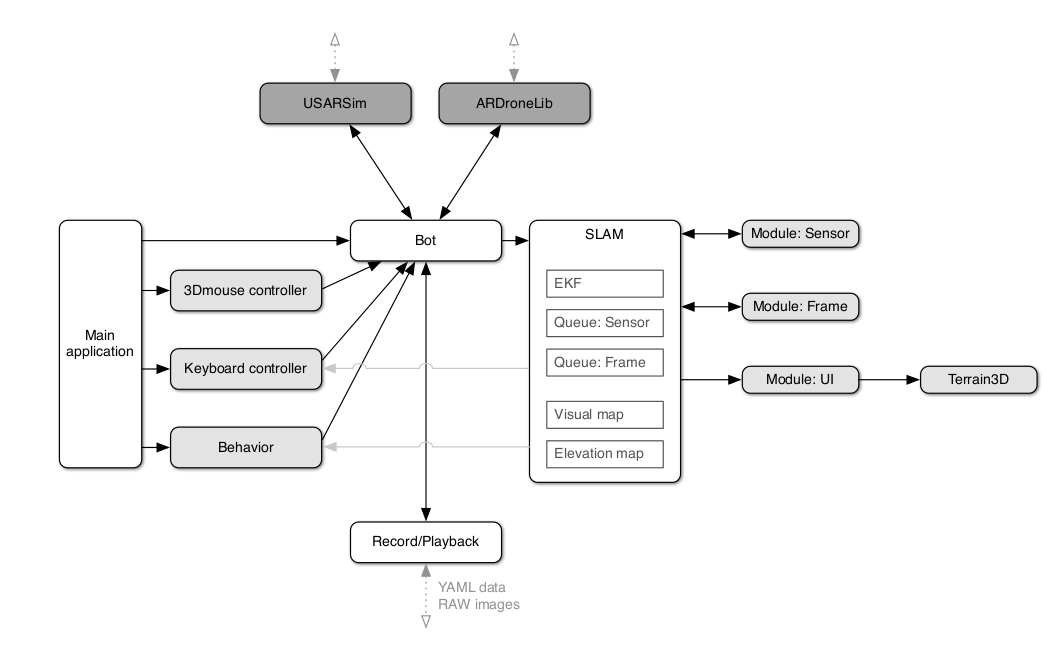
\includegraphics[width=\textwidth]{images/framework.png}
\caption{Schematic overview \cite{Dijkshoorn2012} of the development framework AR.Drone SLAM}
\label{frameworknick}
\end{figure}
\end{appendices}

\newpage

% BIBLIOGRAPHY
\section{Bibliography}
\renewcommand{\section}[2]{}
\bibliographystyle{apalike}
\bibliography{references}
\end{document}